\documentclass[sigconf, anonymous]{acmart}

\fancyhf{} % Remove fancy page headers 
\fancyhead[C]{Anonymous submission \#9999 to ACM CCS 2017} % TODO: replace 9999 with your paper number
\fancyfoot[C]{\thepage}

\setcopyright{none} % No copyright notice required for submissions
\acmConference[Anonymous Submission to ACM CCS 2017]{ACM Conference on Computer and Communications Security}{Due 19 May 2017}{Dallas, Texas}
\acmYear{2017}

\settopmatter{printacmref=false, printccs=true, printfolios=true} % We want page numbers on submissions

%%\ccsPaper{9999} % TODO: replace with your paper number once obtained

\begin{document}
\title{Understanding Real-World Malwares and Anti-Virus Engines}%Template for ACM CCS 2017} % TODO: replace with your title

\begin{abstract}
Your abstract should go here. You will also need to upload a plain-text abstract into the web submission form.
\end{abstract}

% TODO: replace this section with code generated by the tool at https://dl.acm.org/ccs.cfm
\begin{CCSXML}
<ccs2012>
<concept>
<concept_id>10002978.10003029.10011703</concept_id>
<concept_desc>Security and privacy~Usability in security and privacy</concept_desc>
<concept_significance>500</concept_significance>
</concept>
</ccs2012>
\end{CCSXML}

\ccsdesc{Security and privacy~Use https://dl.acm.org/ccs.cfm to generate actual concepts section for your paper}
% -- end of section to replace with generated code

\keywords{template; formatting; pickling} % TODO: replace with your keywords

\maketitle

\section{Introduction}
\label{sec:intro}

There is and will continue to be a constant competition between anti-virus tools and malwares.
Malwares grow exponentially~\cite{avtest} and place an imperative threat to human society. 
For example, more than 390000 new malwares are registered in AVTest institute every day~\cite{avtest}.
As another example, a new type of threat, ransomware, has caused more than 1 billion dollars this year~\cite{ransomware}. 
In order to keep up and detect these new types of malwares, anti-virus tools are also improving rapidly,
by constantly updating their signature database, by using more advanced techniques like deep learning~\cite{cylance}, or by utilizing more data. 

In order to improve anti-virus tools and defend against emerging threats from malwares, 
it is essential to understand malwares and existing anti-virus tools in the real world. 
Previous works on studying malwares and anti-virus engines do provide valuable 
insights~\cite{ZhouSP2012,GuptaComsnets2009, vendors-study} such as  
how malware writers create new malwares and how malwares escape from the detection of anti-virus engines.
However, these previous works only studied limited malwares
%and fail to understand malwares in a large scale, 
and did not provide insights into the relationship between malwares and anti-virus engines. 

We propose to use the vast amount of existing ``big data'' 
to study real-world malwares and their relationship with anti-virus engines.
To conduct such study, we utilized an open data repository
that contains billions of real-world malwares, {\em \vt}.

\vt{} is a free online malware scanning servive
that applies a set of state-of-the-art anti-virus engines to analyze user-submitted files 
and sends a detection report back to user.
\vt{} provides public access to all its submitted files and analysis results. 
\vt{} is a valuable resource to study and 
understand real-world malwares and anti-virus engines. 

First, there are huge amount of suspicious files submitted to VirusTotal. 
%As shown in Figure~\ref{fig:subnum}, 
For example, within our data collection window, 
there were around 40 million submissions to \vt\ each month. 
These submissions cover a large variety of file types, and 
are conducted by a large variety of \vt\ users from all over the world. 
This amount of diverse data on VirusTotal serves as a good representation of malwares in the real world.  

Second, for almost all submissions, 
VirusTotal applies no less than 50 state-of-the-art anti-virus engines to analyze them. 
VirusTotal keeps detailed detection results and provides an open access to these results. 
Analyzing historical detection results can help capture how anti-virus engines evolve over time. 

Third, VirusTotal provides rich metadata for each submission. 
Besides the detection results of various anti-virus engines, 
VirusTotal also provides file type information, submitter information, and a hash string of the original submitted file.
These types of information is valuable to study 
%which can help categorize malwares, 
%source ID (country), which can help understand popularity of malwares, 
%ssdeep digest string, by using which we can calculate code similarity without accessing binary executable, and so on. 

Unfortunately, there has only been limited attention to \vt\ in the past. 
%Researchers have used \vt\ as a testing platform when \yiying{developing malwares?}
Researchers tried to capture malware writers who leverage \vt{} as the testing platform during malware development~\cite{huangvt2016bigdata, neeles}. 
Anti-virus vendors use \vt\ to detect possible false positives and false negatives in their products. 
But none of them study the rich malware data provided by \vt\ in a large scale. 

We collected 4 months of metadata of all submissions to VirusTotal 
and conducted an extensive study on them.
%Following previous works~\cite{SongAPsys2016} on studying VirusTotal,
%We focus our effort on Windows \textit{Portable Executable} ({\em \pe}) files, 
%which account for more than half of \vt{}’s submissions.
After collecting and pre-processing data from \vt, 
we first perform a set of basic analysis to gain an overall knowledge of the \vt\ data repository,
including how big the files submitted to \vt\ are, who submit to \vt, and how many submissions are labeled as malware.

On top of these basic findings, we developed a set of more advanced studies in three directions. 

First, we study the correlation between submissions’ metadata and their {\em detection rates}, 
the percentage of engines labeling a submission as malware. 
We found high correlation between detection rate 
and three factors: submission file size, the history of submitting a file, and the reputation of the submitters.
These results shed light on what types of submission are more likely to be malware.
With this result, future researchers and anti-virus vendors can have more guided direction 
into what they should have further investigation.
%help security experts invest their limited manual efforts, 
%and help anti-virus vendors identify possible false positives and false negatives in their products.   

Second, we study the question of whether or not different anti-virus vendors can influence each other
and if detection rate is a perfect measurement of the likelihood of a file being a true malware.
Anecdotely, anti-virus vendors frequently leverage VirusTotal to identify false negatives in their products, 
which are malwares detected by others’ products but not detected by their own products. 
To verify this hypothesis, we use the detection history from VirusTotal 
and developed statistical models based on a known technique from from the web mining area to quantify the influence between vendors. 
With this method, we confirmed that there do exist high influence between vendors;
certain vendors are highly influenced by the detection results of other vendors and use this information to change their detection results.
This result alerts \vt\ users and researchers to be more careful about the detection results from vendors 
and use detection rate more precautiously.
%Anti-virus vendors can rely on this technique to identify false negatives in their products. 

Third, we explore the feasibility of building malware classifiers or detectors based only on hash values of files.
We obtained hash strings of submitted files to \vt\ 
and use the similarity of these hash string to build classifiers.
%The similarity between two ssdeep hash strings 
%is a good estimation of similarity between the two original binary files.
%If we can build malware detectors by using ssdeep hash strings, 
%we can avoid manually extract signatures from malware samples.   
We design several machine learning experiments to evaluate our hash-based malware classifiers. 
Surprisingly, our evaluation results show that by just using hash string, 
we can obtain high accuracy for certain classification tasks.
At the same time, other classification tasks are not as accurate.
We further developed a mechanism to predict which classification task is likely to have high accuracy.
With these classification and detection mechanisms and the large amount of data,
it will be possible to just use a compressed representation of files instead of the original files 
to detect malware.
This result implies that future users can have higher privacy and do not need to reveal their files to know whether or not they are malware.
%Our evaluation results show that precision of malware classifiers are 
%bounded by percentage of tailing examples and more training data tends to bring better results.

Our study advances the understanding of malwares and anti-virus engines in the real world 
and provides various valuable insights for future researchers and vendors.
%apply machine learning to malware detection in a large scale. 


\section{Empirical Study on how VirusTotal is used in academic papers}

\subsection{How we collect paper and characteristics of collected paper}

In this section, we introduce our findings of how current researchers make use of \vt. 
We collected 101 conference papers by searching \vt\ in Google Scholar. 
They are from many conferences include Usenix Security, NDSS, S\&P, etc. 
\begin{table}
	\label{tbl:literature_confs}
	\caption{The distribution of papers in each conference}
	\begin{tabular}{|c|c|c|}
\hline
Conferences & Count & Topics\\\hline
asia ccs & 12 & security\\\hline
acsac & 11 & security\\\hline
www & 10 & The Web \& information retrieval\\\hline
ccs & 9 & security\\\hline
Usenix Security & 8 & security\\\hline
S\&P & 8 & security\\\hline
NDSS & 7 & security\\\hline
CODaSPY & 6 & Data and security\\\hline
imc & 4 & Measurement \& perf. analysis\\\hline
sac & 4 & \\\hline
eurosec & 3 & security\\\hline
AISec & 3 & security\\\hline
FSE & 2 & Software engineering\\\hline
DSN & 2 & security\\\hline
DIMVA & 2 & security\\\hline
icse & 2 & Software engineering\\\hline
nips & 2 & data\\\hline
ESORICS & 2 & security\\\hline
issta & 2 & Software engineering\\\hline
kdd & 1 & data\\\hline
ase & 1 & Software engineering\\\hline
total & 101 & \\\hline
	\end{tabular}
\end{table}
\begin{table}
	\label{tbl:literature_year}
	\caption{The distribution of papers in each year}
	\begin{tabular}{|c|c|}
\hline
year & count\\\hline
2008 & 1\\\hline
2009 & 4\\\hline
2010 & 2\\\hline
2011 & 4\\\hline
2012 & 6\\\hline
2013 & 13\\\hline
2014 & 21\\\hline
2015 & 12\\\hline
2016 & 15\\\hline
2017 & 17\\\hline
2018 & 6\\\hline
\end{tabular}
\end{table}

The number of papers from each conference is listed in Table~\ref{tbl:literature_confs}. 
Their publication year ranges from 2008 to 2018. The detailed distributions is listed in Table~\ref{tbl:literature_year}.

c. Topic distribution 

The papers cover a large range of topics. 
Many of them are related to the detection or techniques of malwares, such as Android apps \cite{arp2014drebin,huangvt2016bigdata}, ransomware \cite{kharraz2016unveil} and Flash \cite{ford2009analyzing}. 
They mainly use \vt's detection results as baseline or ground truth. 
There are 89 papers use \vt\ to label or collect data set among the 101 papers. 
The rest 13 papers mention \vt\ for other purposes. 
We mainly focus on how the 89 papers use the detection result of \vt.

There several issues that researchers need to consider in using the results. 
First, researchers could collect detection results from multiple vendors. 
It is necessary to aggregate the results into one as the label of malware or benign for some works. 
We would like to know how researchers aggregate them. 
Second, the detection results could change over time and it is more reliable to collect the results from \vt\ during a period of time. 
We would also like to know the practice on collecting results from \vt\ over time. 
Thrid, vendors could have different impacts. 
It is also interesting to know whether and how researchers considered the different impacts of vendors.

%Last but not least, it is worth considering how we merge results from different vendors. 
First, we look at how researchers merge detection results. 
In most cases, researchers get results from more than 40 or 50 vendors and merge the results as one for their dataset. 
There are mainly two ways of merging: 1) considering a submission as malicious if any vendor can detect; 2) considering a ratio or a threshold for the number of vendors. 
For instance, Ford et al. \cite{ford2009analyzing} report it as malicious as long as there is a vendor reporting malicious
towards a file, while Carmony et al. use a threshold of 15 files. 
Among the 89 papers, 26 papers (29.2\%) use the first way and 46 papers  (51.7\%) use the second way. 
The rest 17 papers (19.1\%) do not mention how they merge results from different vendors.

Second, there are only 4 papers (4.5\%) consider that the detection results could change over time, and collect the results from \vt\ during a period of time. 
The length of time could vary from several days \cite{kharraz2016unveil, rajab2013camp} to months \cite{neeles, wressnegger2017looking}. 

Third, among the 89 papers, only 8 papers (9.0\%) consider that different vendors shall have different impact. 
Most of them pick out three to more than ten vendors to discuss their impact, because of their influence in industry or good performance on detection rate. 
For instance, Arp et al. \cite{arp2014drebin} inspected the output of ten vendors and list their detection rate anonymously. 
In addition, all of the papers treat the vendors equally. %Thomas et al. \cite{thomas2015ad} listed detection rate of 3 vendors. 
\subsection{Findings}
a. Do not wait until results become stable

b. Treat vendors equally

\subsection{Discussion}
What if the current usage is not correct? 

\section{Data Collection}%Methodology to collect VirusTotal data}

%\subsection{The large data set}

%How the data set is built?

%What information we can get? Basically, we need to explain the data format. 

%Basic properties of the data set

%a. How many submissions every data?

%b. Submission type distribution

%c. The number of submissions for the same file

%d. Engines used to scan a submission 

%Advantage: 

%Across categorization, such as file types 

%Covering a longer time.

In this section, we introduce how we collect data. 

\subsection{Methodology}

First, we introduce our data source, VirusTotal, and how we make use of their APIs. VirusTotal offers a lot of APIs for researchers. Their private APIs could return the detailed detection results of vendors. We applied for a private API key for our data collection. We mainly use two APIs for collecting data: \texttt{report} and \texttt{rescan}. \texttt{report} takes a hash value of a sample as input, and returns a detailed report of the sample if the sample exists in the library of VirusTotal. The report contains the detection results of the sample from all the vendors that VirusTotal could provide. \texttt{rescan} also takes a hash value as input. This API sets VirusTotal to rescan the specified sample. This could make VirusTotal to update the detection results of samples.

Then we introduce how to collect the data set. 
First, at day 0, we obtained about 14,423 new Portable Executable (PE, the executable file format on Windows) files from an anti-virus vendor. 
We then submitted the 14423 files to VirusTotal at the same day, and got the detection results from VirusTotal. 
None of these files were submitted to VirusTotal prior to day 0.
For each day later on, we first call \texttt{rescan} on the 14423 files respectively. Then, we wait 2 hours for VirusTotal updating the detection results. 
After 2 hours, we call \texttt{report} on each files to get the updated detection results. 
We keep collecting data for 75 days. 

\subsection{What information can we get from VirusTotal?}% I mean the data format. 

The API \texttt{report} returns a lot of information of the sample, including but not limited to hashcodes (MD5, SHA1, etc.) of the sample, scan date, and detailed scan results of many vendors. For each vendor in the detailed scan results, there are 4 fields: \texttt{detected}, \texttt{version}, \texttt{result}, and \texttt{update}. \vt\ does not provide detailed documentation of the fields, but it is easy to infer from the results and other documents (such as https://www.virustotal.com/en/faq/). \texttt{detected} tells if the sample is detected as malicious by this vendor. \texttt{version} tells the version used in the scan. \texttt{result} is how the vendor classifies the sample. \texttt{update} is the date of the vendor providing the anti-virus tool.

\subsection{Basic properties of the data set}

Now we take a look at the data set. First, there are 7197 malicious files and 7226 benign files according to the results from first scan. We say ``malicious'' as long as there is one vendor reporting malicious. This indicates that our dataset is balanced.

Then we check the completeness of the dataset by observing two distributions. 
Our dataset could be regarded as a set of tuples $(f, v, t)$ that sample $f$ is scanned at time $t$ by vendor $v$. Ideally, there should be one tuple for all $f, v, $ and $t$ in all 14423 files, more than 70 vendors and 75 days. 
However, not all valid tuples exist in the downloaded information. Some tuples may miss because of VirusTotal or our crawling configuration. So we calculated two distributions of the data set to check the completeness.
First, Figure~\ref{fig:dataset_submission_vendor_distri} shows the distribution of how many vendors have scanned a sample in a detection result. A point $(x, y)$ on the curve represents that there are $y$ detection results with $x$ vendors scanned. From the chart, we can know that most of the detection results are detected by more than 65 vendors. 
In addition, Figure~\ref{fig:dataset_no_vendors_scanned_moste_files_in_x_days} shows  how many vendors scan most of the files in how many days. More specifically, $(x, y)$ in the chart represents there are $y$ vendors that scans more than 90\% of the total files in $x$ days. The figure indicates that most of the vendors 
From the two figures, we could conclude that the dataset is mostly complete.

\begin{figure}
\centering
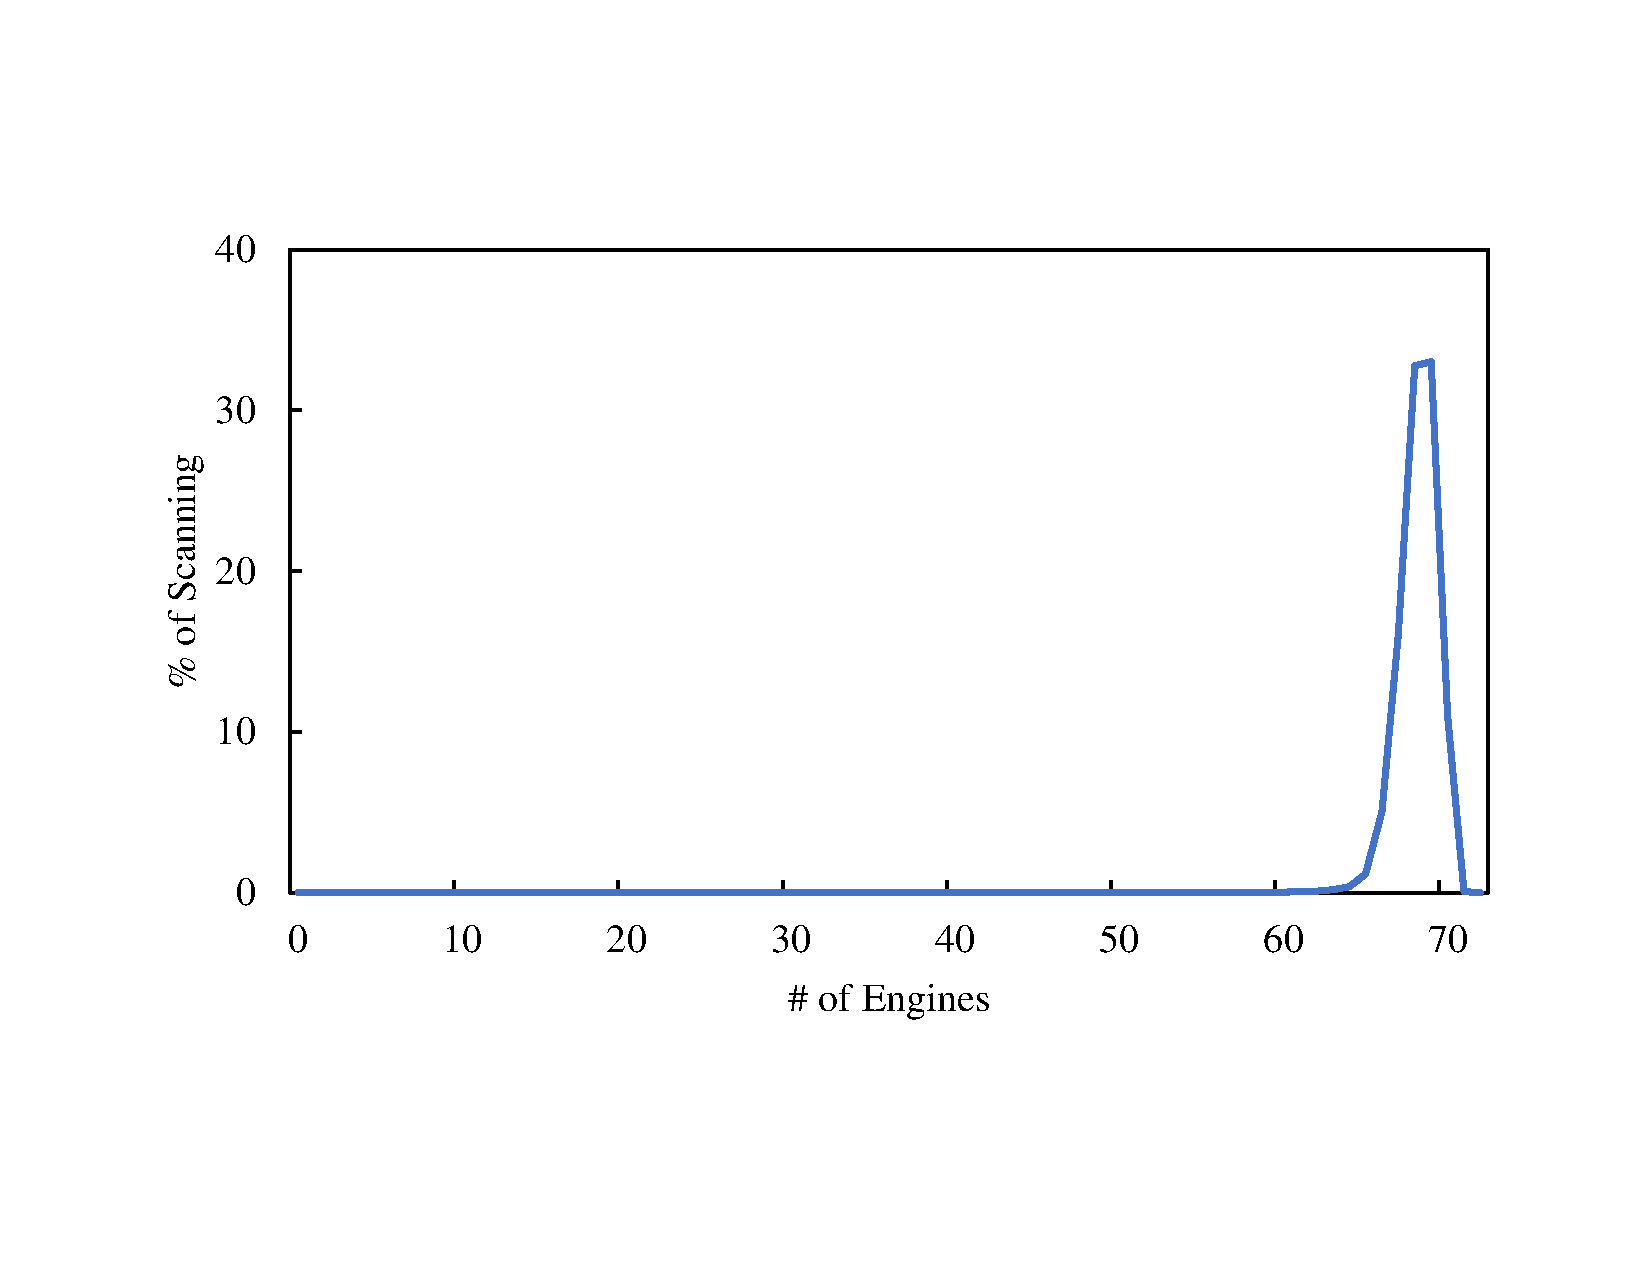
\includegraphics[width=0.7\linewidth]{figure/vendor_submission_distribution}
\caption{Distribution of detection results vs. vendors}
\label{fig:dataset_submission_vendor_distri}
\end{figure}

\begin{figure}
\centering
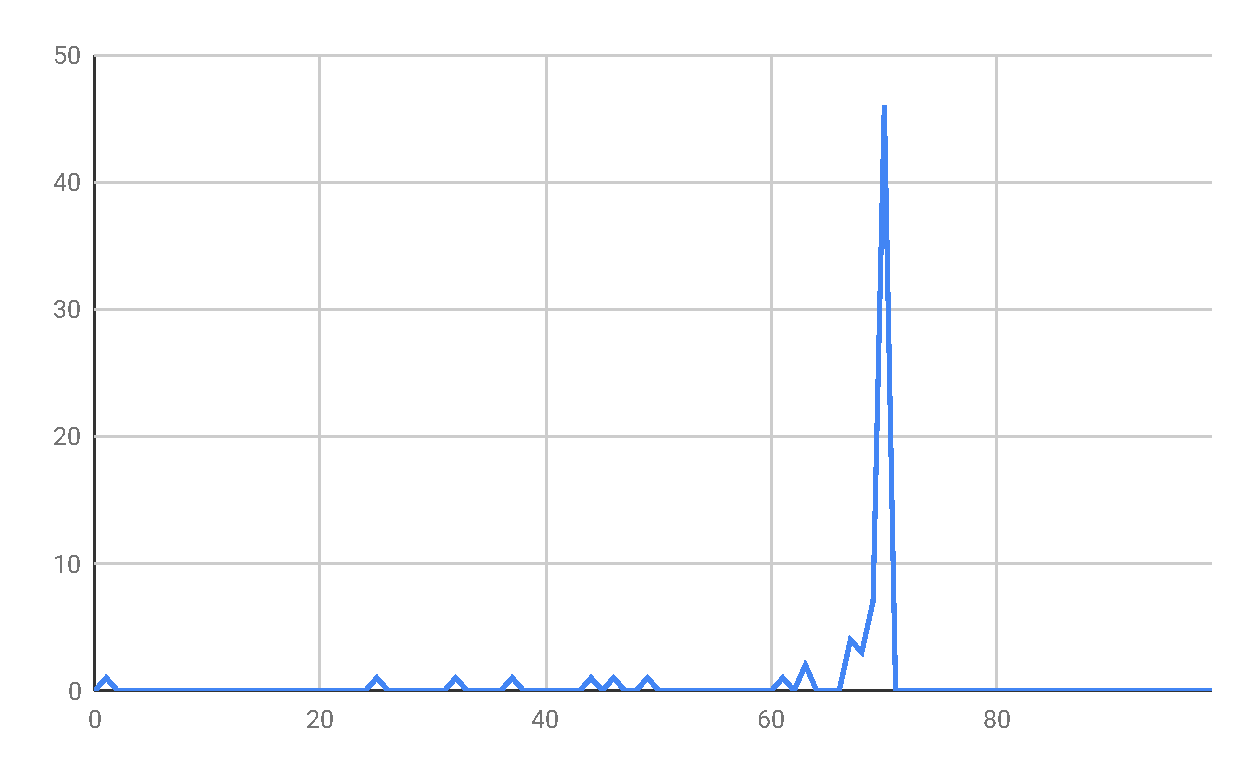
\includegraphics[width=0.7\linewidth]{figure/dataset_no_vendors_scanned_moste_files_in_x_days}
\caption{the number of vendors that scanned more than 12980 (>90\%) files in $x$ days}
\label{fig:dataset_no_vendors_scanned_moste_files_in_x_days}
\end{figure}


\subsection{How VirusTotal update engines?}
As we mentioned above, we use \texttt{rescan} and \texttt{report} to get the latest detection results from VirusTotal for each day. Actually, how VirtusTotal update the antivirus engines? With our data set for 75 days, we first check whether antivirus bases and versions update over time. We find that more than 78\% of the detection results updates consistently with time went on. So we can get new detection results from VirusTotal when we \texttt{rescan} samples and \texttt{report} detction results 2 hours later.


\begin{figure}
\centering
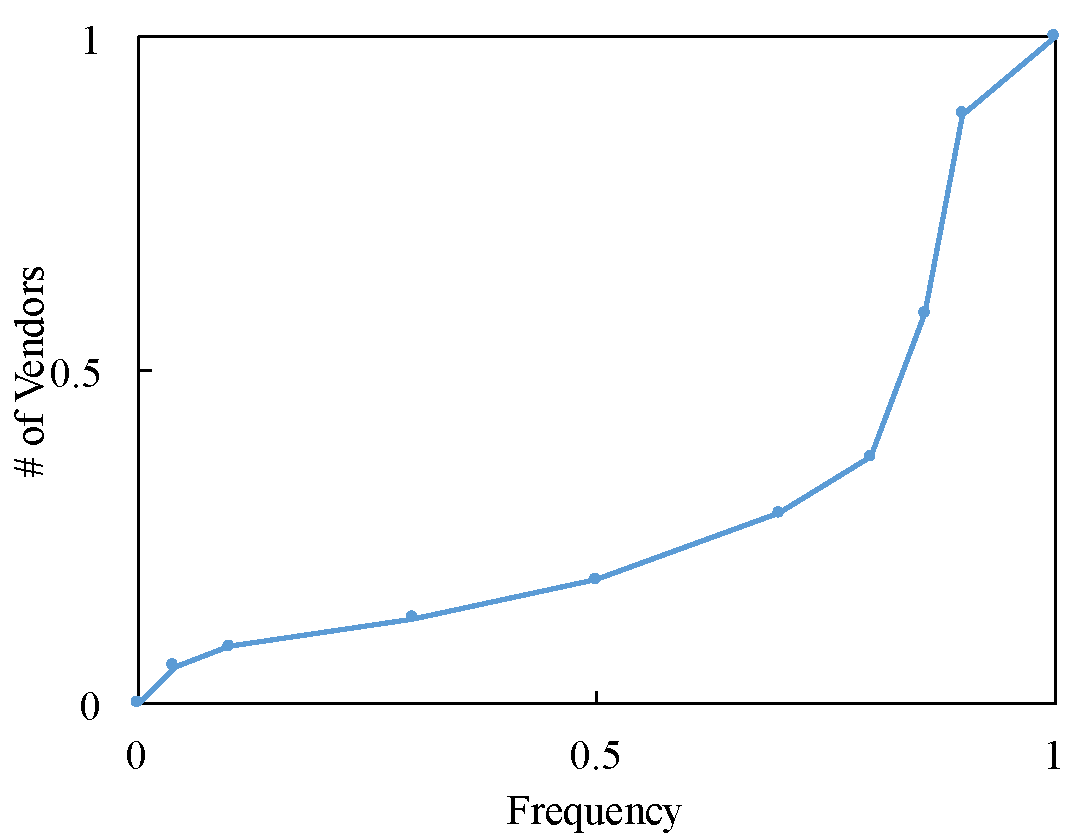
\includegraphics[width=0.7\linewidth]{figure/frequency}
\caption{Distribution of update frequency over vendors.}
\label{fig:frequency}
\end{figure}

Figure \ref{fig:requency} presents the distribution of updating frequency for vendors. Overall, more than 44 vendors(total 70) update their detction results with at least 1 day. Only 6 vendors' updating frequency are less than 0.05, and 4 of them seems not change their antivirus engines during these 75 days. Averagely, about 56 vendors will be updated with at least 2 days. 

%c. How VirusTotal update engines? Scanning time vs. update vs. version 
%TODO: need more data
\subsection{Caveats}

Discuss errors during our data collection. 

\section{Flipping and stable study}

In this section, we present how we analyze our collected data during these 75 days, and try to find some patterns on the detection results of 14423 samples from 70 vendors. 

Based on our obversation, we first give some definitions of different patterns: (1) Stable pattern: This pattern means that the detection results of a file from an vendor or all vendors would never change. (2)Flip pattern: Some vendors will change the detection result of a file from malicious to benign or from benign to malicious one time in the sequence. (3)Hazard pattern: The results would be updated from benign to malicious at one day, and then back to benign again. The same situation would also happen on malicious files. 


\subsection{Hazard discussion}

\begin{figure*}[!htb]
\minipage{0.31\textwidth}
  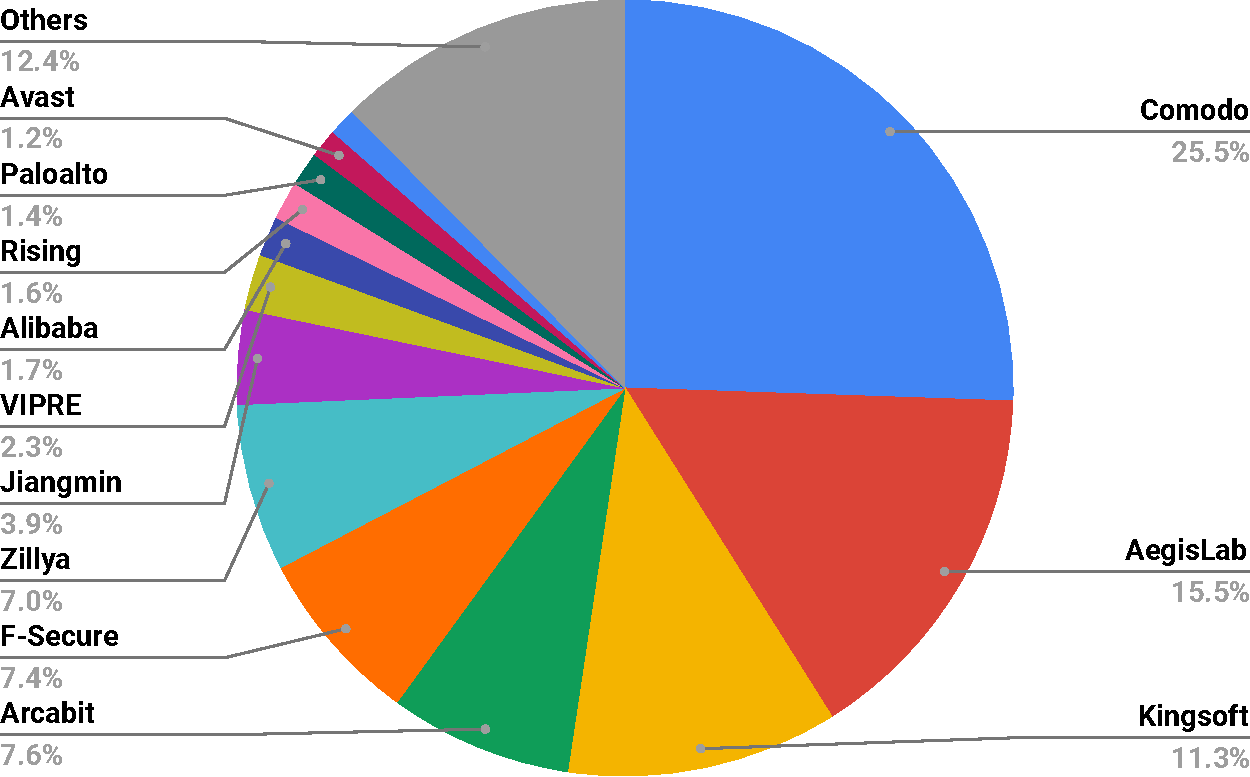
\includegraphics[width=\linewidth]{figure/hazard_vendorAll}
  \caption{Hazard distributions for vendors.
%(File types and their distributions for all VirusTotal submissions from 05/07/2016 to 09/06/2016.)
}
\label{fig:hazard_vendorAll}
  %\label{fig:overlap}
\endminipage\hfill
\minipage{0.31\textwidth}
  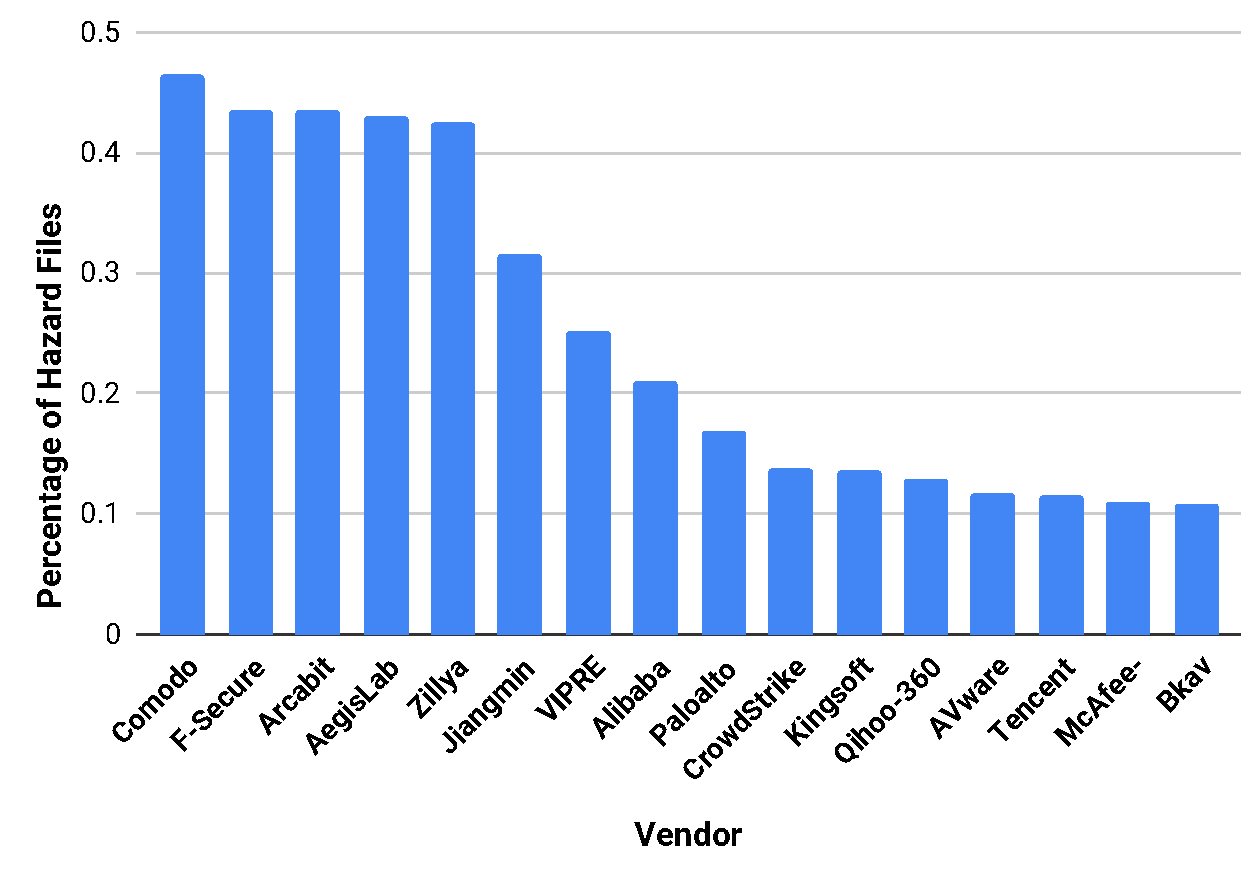
\includegraphics[width=\linewidth]{figure/hazard_vendorFile}
 \caption{Hazard file distributions for per vendor.
%{\footnotesize{
%(The number of suspicious files and the number of PE files submitted to VirusTotal from 05/07/2016 to 09/06/2016.)
%}
}
\label{fig:hazard_vendorFile}
  %\label{fig:maxUncover}
\endminipage\hfill
\minipage{0.31\textwidth}%
  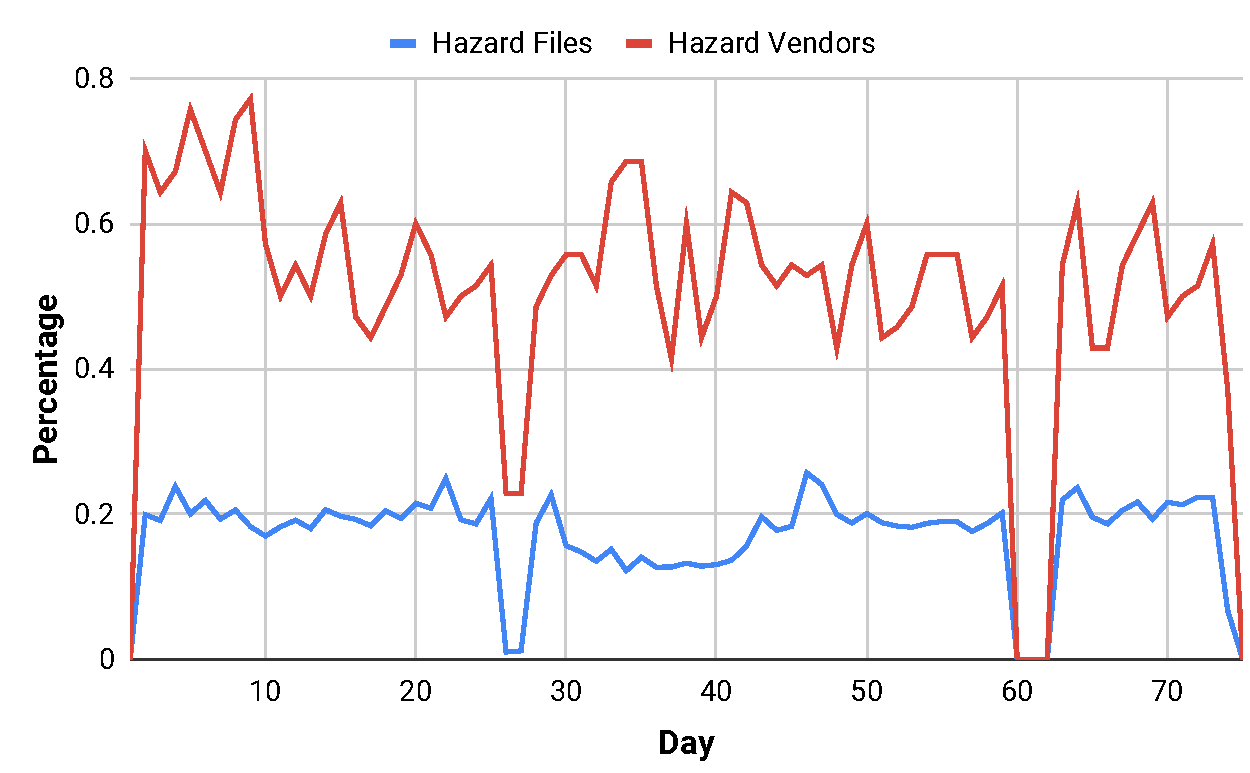
\includegraphics[width=\linewidth]{figure/hazard_day}
\caption{Hazard file and vendor distributions for per day.
%\footnotesize{
%(Only countries with more than 1\% PE submissions are shown.)
%}
}
\label{fig:hazard_day}
\endminipage\hfill

%\vspace{-0.2in}
\end{figure*}

Hazard pattern is an abnormal situation in the dection result sequences. It could affect the study of the other two patterns. So we first caculated the distribution of hazards over vendors, sampling files and days in our original data set.

In our statistics, only 3 vendors have no hazard patterns and other 67 vendors have hazards with different percentage. Hazards from the top 3 vendors accounts half of hazards and 13 vendors can cover more than 87\% hazards. Other 54 vendors have less than 1\% hazards, as shown in Figure \ref{fig:hazard_vendorAll}. Hazard pattern is quite frequently among vendors and sampling files.

Figure \ref{fig:hazard_vendorFile} shows the percentage of hazard files from top 16 vendors. Other vendors contains less than 10\% hazard files. "Comodo" contains the most hazards but has less than half of hazard files. We can make a conclusion from these results that hazard pattern is not caused by the engine misfunction. 

Figure \ref{fig:hazard_day} plots hazards distribution of files and vendors over every day. Overall, we find that hazard files randomly appear almost every day during these 75 days. The same conclusion can be made to hazard vendors. 

Figure \ref{fig:hazard_fileVendor} presents hazard file distribution over vendors. Only 4 hazard files involves more than 30 vendors and we did not find a file that its detection results from 70 vendors have hazard patterns. Thus, hazard pattern may not caused by the VirusTotal API.



%Todo: add hazard discussion in this part before discussing flipping. 

%Hazard caused by VT API? NO

%Hazard caused by vendor misfunction? NO

%conclusion: randomly appear, but quite frequently, affect lots of files

%Conclusion: remove hazard before studying flipping?

%Run experiments both with and without hazard
\textbf{Summary:} Hazard pattern is obviously common in our results and it affects lots of files and vendors. An immediate question that follows is what the results would be if we remove hazards before studying flipping and stable patterns? We will give more explanations of our experiments in the following sections.  

\subsection{Flipping Study}
%a. For each file, we count  of flipping vendors and  of flipping times

\begin{figure*}[!htb]
\minipage{0.31\textwidth}
  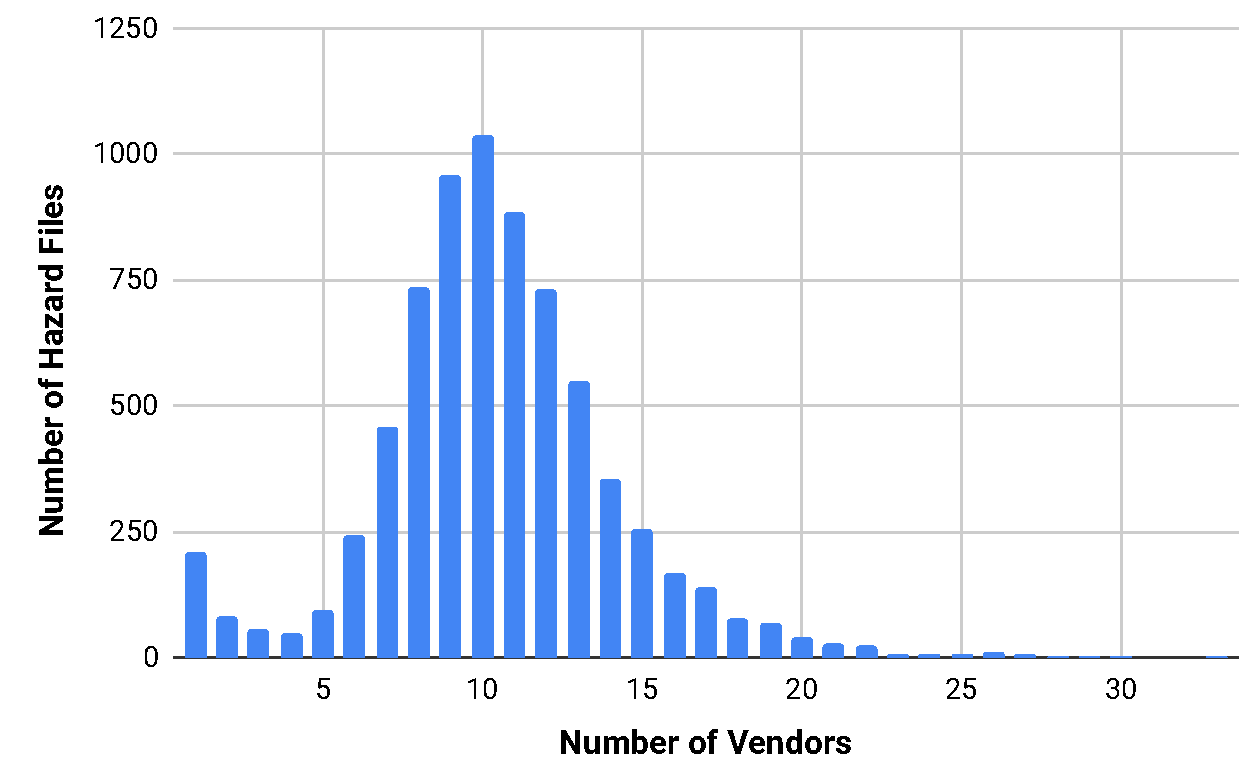
\includegraphics[width=\linewidth]{figure/hazard_fileVendor}
  \caption{Hazard file distributions over vendors.
%(File types and their distributions for all VirusTotal submissions from 05/07/2016 to 09/06/2016.)
}
\label{fig:hazard_fileVendor}
  %\label{fig:overlap}
\endminipage\hfill
\minipage{0.31\textwidth}
  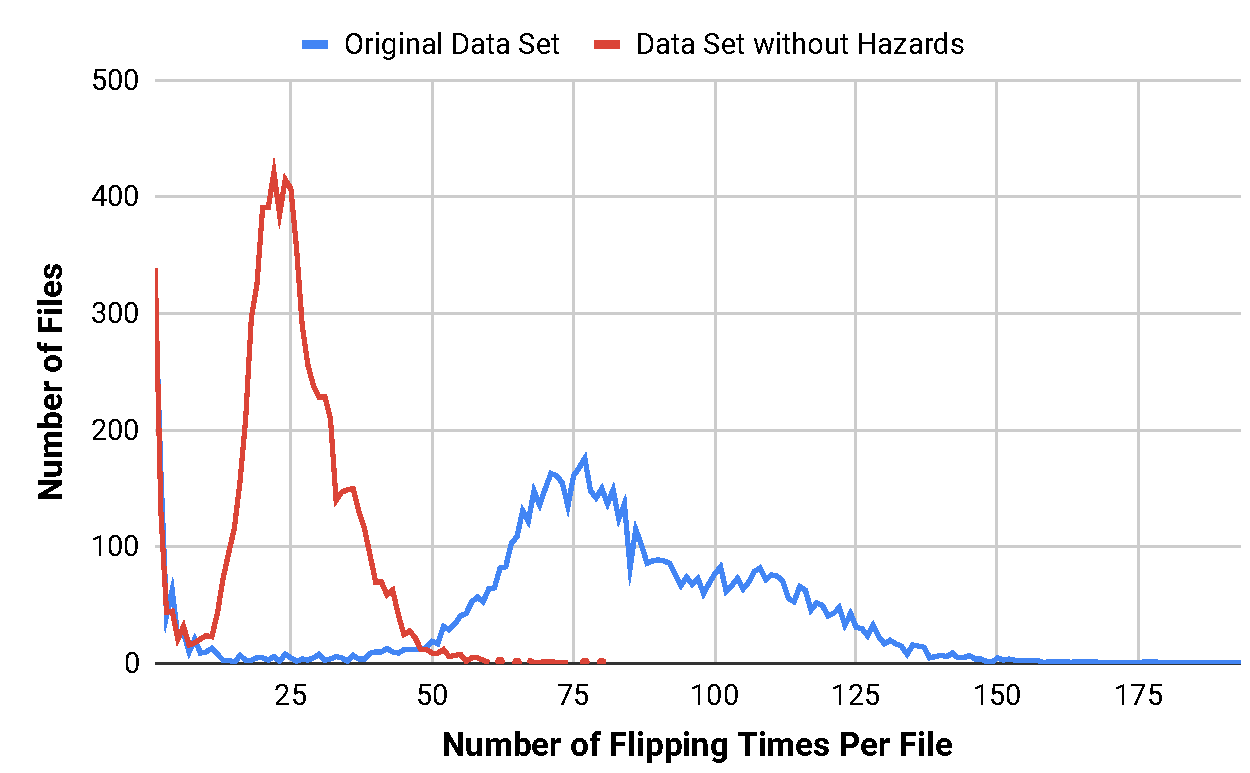
\includegraphics[width=\linewidth]{figure/flip_all}
 \caption{Flipping distributions for per file.
%{\footnotesize{
(The number of flipping times comparisons on data set both with and without hazards.)
%}
}
\label{fig:flip_all}
  %\label{fig:maxUncover}
\endminipage\hfill
\minipage{0.31\textwidth}%
  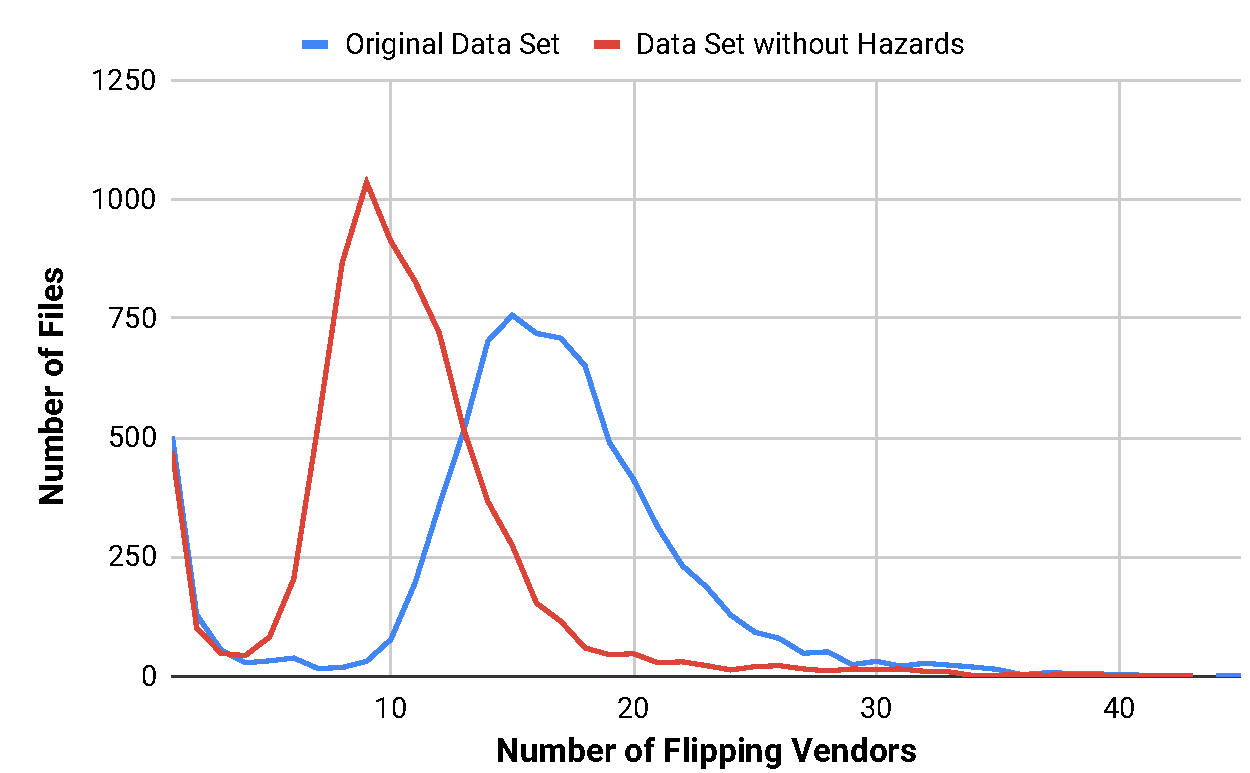
\includegraphics[width=\linewidth]{figure/flip_file}
\caption{Flipping vendor distributions for per file.
%\footnotesize{
(The number of flipping vendors comparisons on data set both with and without hazards.)
%}
}
\label{fig:flip_file}
\endminipage\hfill

%\vspace{-0.2in}
\end{figure*}

This section presents our results of flipping pattern study. As we discussed above, flipping pattern is an important pattern that affects a file to be stable. To study the flipping pattern, we calculate fippling distribution over files and vendors respectively in our original data set. Then, we remove hazards from our data set and recaulate the distributions for further comparison. 

Figure \ref{fig:flip_all} shows the distribution of flipping times for each file. Totally, we find that 7754 files have flipping patterns(total 14423), and the number drops to 7657 after smoothing hazards. Only 1 file have the largest flipping times of 193, and most files have only one flip. Without hazards, the largest flipping times is 80 and most files contian less flippings. For example, more than 421 files contain 22 flipping patterns. We can make the similar conclusion from the distribution of flipping vendors for each file, as shown in Figure \ref{fig:flip_file}. 

%b. For each vendor, we count  of flipping,  of flipping files, average flipping per file

To figure out the distribution of flipping pattern for each vendor, we calculate the flipping times, the number of flipping files from each vendor and the average flipping times per file. We run the same experiments both on our original data set and data set without hazards.

Overall, 68 vendors have flipping patterns(total 70), and "Comodo" contains more flipping patterns than other vendors. Some vendors, such as "Avast-Mobile" and "eGambit", have no flippings during the detction period. We present top 16 vendors ranking in the flipping list in Figure \ref{fig:flip_vendorAll}. Compared with results from the original data set, removing hazards has greatly reduced the flipping times for each vendor. 

Figure \ref{fig:flip_vendorFile} shows the distribution of flipping files for each vendor. 7 vendors have more than 40 percentage fippling files(total 14423). Removing hazards almostly does not affect the number of flipping files of some vendors. For some vendors, such as "Acrabit", "Zillya", "F-Secure", "CrowdStrike", we find the number of flipping files dramatically drops when we remove hazards from the original data set.

Figure \ref{fig:flip_vedorAvg} plots the average flipping times of a file from each vendor. We present 28 vendors that have more than 2 flipping times per file averagely, while other 42 vendors hold less than 2 flippings for each file. The most frequent flipping happens on "Comodo". On average, it contains more than 30 flipping times per file. Without hazards, the average flipping times significantly fall into almost half of original results. 

\begin{figure*}[!htb]
\minipage{0.31\textwidth}
  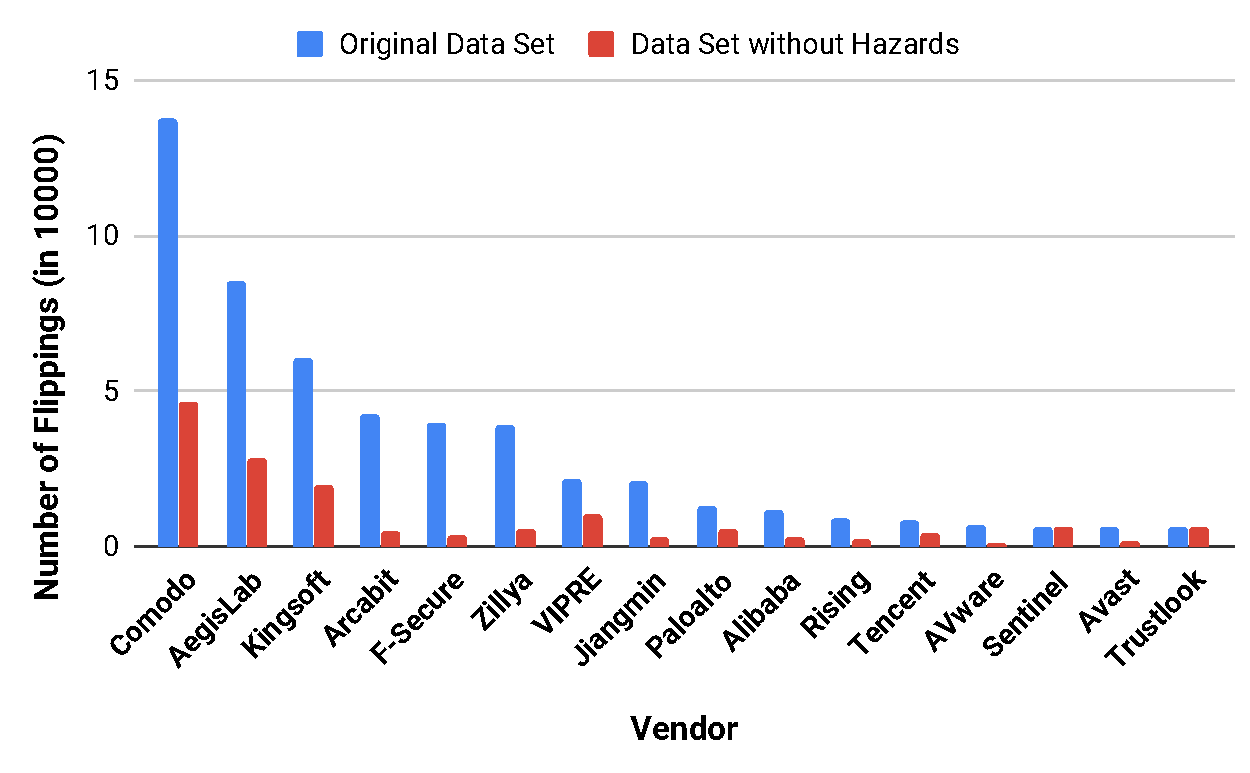
\includegraphics[width=\linewidth]{figure/flip_vendorAll}
  \caption{Flipping distributions for vendors.
(The number of flipping times for per vendor comparisons with and without hazards.)
}
\label{fig:flip_vendorAll}
  %\label{fig:overlap}
\endminipage\hfill
\minipage{0.31\textwidth}
  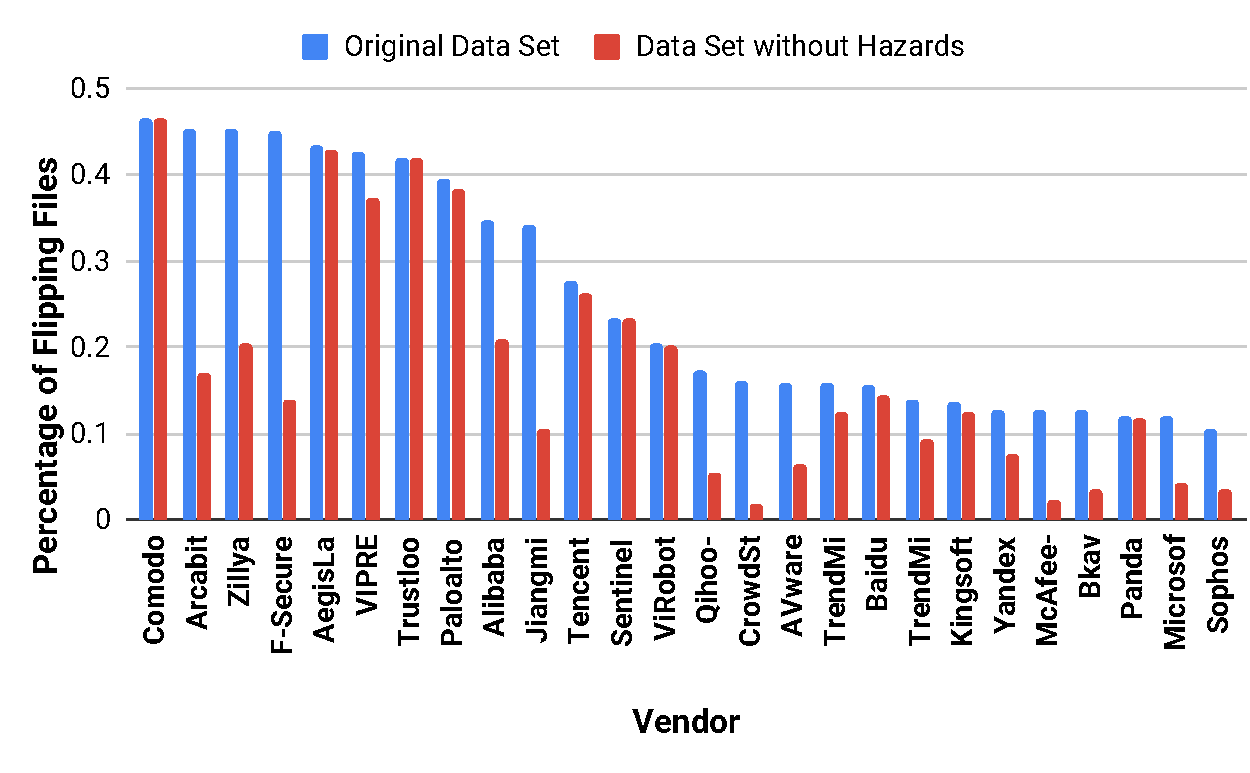
\includegraphics[width=\linewidth]{figure/flip_vendorFile}
 \caption{Flipping file distributions for per vendor.
%{\footnotesize{
(The number of flippings files for per vendor comparisons with and without hazards.)
%}
}
\label{fig:flip_vendorFile}
  %\label{fig:maxUncover}
\endminipage\hfill
\minipage{0.31\textwidth}%
  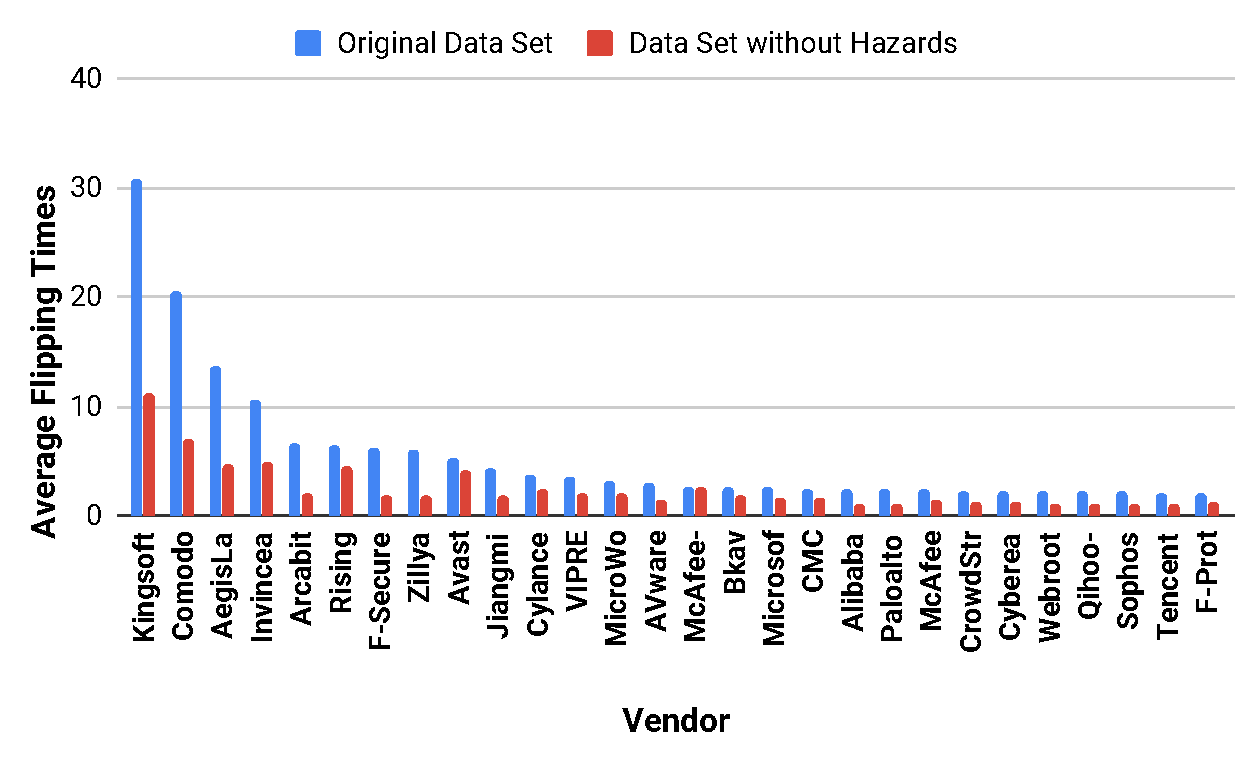
\includegraphics[width=\linewidth]{figure/flip_vendorAvg}
\caption{Average flipping times of a file for per vendor.
%\footnotesize{
(The average flipping times of a file for per vendor comparisons with and without hazards.)
%}
}
\label{fig:flip_vedorAvg}
\endminipage\hfill

%\vspace{-0.2in}
\end{figure*}

\textbf{Summary:} Flipping pattern widely exists in our experiments. Statistically, more than 50\% files and 97\% vendors have flipping patterns. Removing hazards is an effective approach to reduce flipping patterns for some vendors, but only 97 files have no flipping pattern after smoothing hazards. A large numbers of files and vendors still have flipping patterns. Flipping pattern is the most important reason that results in many files and vendors to be unstable.


\subsection{Stable Study}
a. We need some metrics to support our definition of ?stable? is reasonable.

b. Some metrics to show how long we need to wait until results become stable

\subsection{Conclusions}

\section{Influence Among Anti-Virus Engines}
\label{sec:influ}

Anti-virus vendors frequently use VirusTotal to identify false negatives in their products, 
which are malware they fail to detect but detected by other vendors~\cite{vt-usage}.
As discussed in Section~\ref{sec:meth}, many files are submitted to VirusTotal more than once, 
and more than 99\% submissions are analyzed by at least 50 anti-virus engines. 
Interestingly, we observe that some engines fail to identify some malware during early submissions, 
but they catch up when analyzing later submissions.

This observation led us to ask one important question that have never been studied before:
{\em is there influence across different anti-virus vendors?}
That is, can an anti-virus vendor's decision be affected by other vendors' malware detection results?
With the large number of anti-virus engines in the wild, it is important to understand if an anti-virus engine is
reliable and can be trusted.  

This section presents our answer to this question by quantifying the influence across anti-virus engines.
Specifically, we study the historical submissions of a file and
how anti-virus engines change their labels of the same file over time.
We also provide a prediction model on whether an engine will identify a file as malware in the future
after labeling the file as benign---a warning flag that this engine's decision is highly likely to be resulted from the influence of other engines.

\subsection{Influence Graph}
\label{sec:model}
We now discuss our proposed mechanism to analyze the influence among anti-virus engines.
Our goal is to estimate the {\em trustworthiness} of an anti-virus engine $i$, $T_i$.

We propose to model the anti-virus engine influence problem as a graph problem.
Influence propagation in social networks is a well-studied topic in the web mining area. 
Inspired by social graph solutions~\cite{Influence}, we propose to use graphs to represent the relationship between vendors 
and model influence among different vendors based on static models.
% first overview static models in our usage scenario,
%and then we discuss how we evaluate static models on data we collect. 

We first build a complete directed graph $G = (V, E)$ called {\em influence graph} for the influence problem, 
where the nodes $V$ are vendors and edges model the likelihood of influence between two vendors. 
We choose to use a complete graph because we initially assume that it is possible to have influence from one vendor to any other vendor.

We use {\em action} to describe the detection result of an engine to a submission. Since a file can be
submitted more than once and an engine can analyze it multiple times, we need to associate action with
time. We formally define an action, $a$, at time $t$ as $(u, a, t)$ or $(u, \bar{a}, t)$,
where the former represents an anti-virus engine identifies the submission as malware 
and the latter represents it identifies the submission as benign.

We limit the goal of this study to detecting whether or not a vendor changes its labeling of a file from
benign to malware because other vendor(s) have labeled it as malware (what we call {\em positive influence}). 
%This is because {\color{red} vendors detecting malware earlier are more trustworthy than vendors following others.}
Thus, we do not consider the case of changing from labeling malware to benign ({\em negative influence}). 
We also assume that after a vendor labels a file as malware it will not change its decision.
A similar model can be applied to study negative influence and we leave it for future work.

We associate each edge $(u, v) \in E$ in the graph $G$ 
with an {\em influence probability} $p_{u,v}$,
which represents the probability that after $u$ takes an action $v$ will follow $u$ to take the same action.
Since we only consider positive influence, 
when calculating $p_{u,v}$, we only consider cases where after $u$ has labeled a submission as malware, 
$v$ will change its label from benign to malware in a later time, i.e., 
$\exists$  $(u, a, t_1)$, $(v, \bar{a}, t_2)$, $(v, a, t_3)$ where $t_1<t_3$ and $t_3>t_2$. 


%\yiying{does this action include both turning from labeling benign to malware and from malware to benign? 
%does it include the first label (no prior labeling by the same node)? you need to explain what an "action" is.}
%Since the graph is a complete graph, 
%all other nodes are all $v$'s neighbors. 

To capture the engines influence an engine, we use the neighbor relationship in the influence graph. 
We define $S_v(a)$ to be the set of $v$'s neighbors that take action $a$ before $v$ in time. 
The probability that $v$ will follow its neighbors to take the same action can then be calculated as:

\begin{equation} \label{eq:setp}
%$$p_v(S_v(a)) = 1 - \prod\limits_{u \in S_v(a)}(1 - p_{u,v})$$
p_v(S_v(a)) = 1 - \prod\limits_{u \in S_v(a)}(1 - p_{u,v})
\end{equation}

We can use $p_{u,v}$ to further estimate the trustworthiness of an engine, $T_v$.
Intuitively, if an anti-virus engine gets more influence from others,
it is less reliable and trustworthy. Thus, we have

\begin{equation} \label{eq:trust}
T_v = \frac{1}{\sum\limits_{u \neq v}{p_{u,v}}}
\end{equation}


\subsection{Influence Probability Estimation Model}
\label{sec:influenceprob}
From the above analysis, we can see that the influence probability is the key of our anti-virus engine
influence problem.
After knowing the value of the influence probability $p_{u,v}$ between all engine pairs $u$ and $v$,
it is easy to calculate the trustworthiness of all engines.
The problem now boils down to estimating $p_{u,v}$.

To estimate the influence probability between two engines, we propose to use the statistics of actions taken by
an engine on a file and the action propagation between two engines. 
Specifically, we use the {\em happen-after} relationship to
define {\em action propagation}; if an action of an engine is taken after an action of another engine, we say that
this action is propagated.

To assist the definition of action propagation, we first define a few types of submission sets.
We use $A_u$ to represent the set of submissions ever identified by $u$ as malware in its history
and $\bar{A}_u$ to represent the set of submissions that have been labeled as benign and yet not labeled as malware by $u$.
%the number of actions taken by $u$, 
%or the number of malware identified by $u$. 
%\yiying{I think all these $A$ should be a collection/set, not the total number, since you use $\in$ later}
%\yiying{Verify that the above sentence is correct.}
Further, we define the set of actions taken by both $u$ and $v$ as $A_{u\&v}$ 
and the set of actions taken by either $u$ or $v$ as $A_{u|v}$.
Thus, $|A_{u|v}| =   |A_u| + |A_v| - |A_{u\&v}|$.
With these sets defined, we formally
define {\em action propagation} in the following equation 
and use $A_{u2v}$ to represent the set of all the actions that are propagated from $u$ to $v$. 

%\begin{definition}{Action Propagation:}
{Action Propagation:}
An action $a$ propagated from $u$ to $v$ iff: (i) $\exists$ $(v, \bar{a}, t_i)$ $\in$ $\bar{A}_v$ 
and $(v, a, t_k)$ $\in$ $A_v$, with $t_i < t_k$; (ii) $\exists$ $(u, a, t_j)$ $\in$ $A_u$, with $t_j < t_k$ and $u \neq v$. 
%\end{definition}

With these definitions, we now present our four proposed static models to estimate $p_{u,v}$.

{\bf Bernoulli distribution} estimates $p_{u,v}$ as the ratio of the number of actions 
propagated from $u$ to $v$ over the total number of actions taken by $u$.

$$p_{u,v} = \frac{|A_{u2v}|}{|A_u|}$$ 

{\bf Jaccard index} estimates 
$p_{u,v}$ as the number of actions propagated from $u$ to $v$ divided by 
the number of actions taken either by $u$ or by $v$.

$$p_{u,v} = \frac{|A_{u2v}|}{|A_{u|v}|}$$ 

On top of the Bernoulli distribution and the Jaccord index,
we add an additional consideration called {\em partial credit}.
When $v$ takes an action $a$, it may be influenced by the combination of all its neighbors $S_v(a)$ 
taking the action $a$ before $v$. %Partial credit takes this intuition. 
To account for this effect, we use partial credit 
and calculate the partial credit for $u$ who takes an action $a$ before $v$ as 

$$credit_{u,v}(a) = \frac{1}{|S_v(a)|}$$

{\bf Bernoulli distribution with partial credit} 
estimates $p_{u,v}$ as the sum of all partial credits taking by $u$ for actions propagated from $u$ to $v$, 
dividing by the number of actions taken by $u$. 

$$p_{u,v} = \frac{\sum\limits_{a \in A_{u2v}}{credit_{u,v}(a)}}{|A_u|}$$

{\bf Jaccard index with partial credit} 
estimates $p_{u,v}$ as the sum of all partial credits taking by $u$ for actions propagated from $u$ to $v$, 
dividing by the number of actions taken either by $u$ or by $v$. 

$$p_{u,v} = \frac{\sum\limits_{a \in A_{u2v}}{credit_{u,v}(a)}}{|A_{u|v}|}$$


Since $|A_{u|v}|$ is not less than $|A_u|$, 
$p_{u,v}$ calculated by Jaccard index is not larger than $p_{u,v}$ calculated by Bernoulli distribution. 
For Bernoulli distribution and Jaccard index, 
considering partial credit will decrease $p_{u,v}$ calculated by both of them. 

\begin{figure*}
\centering
\subfloat[]{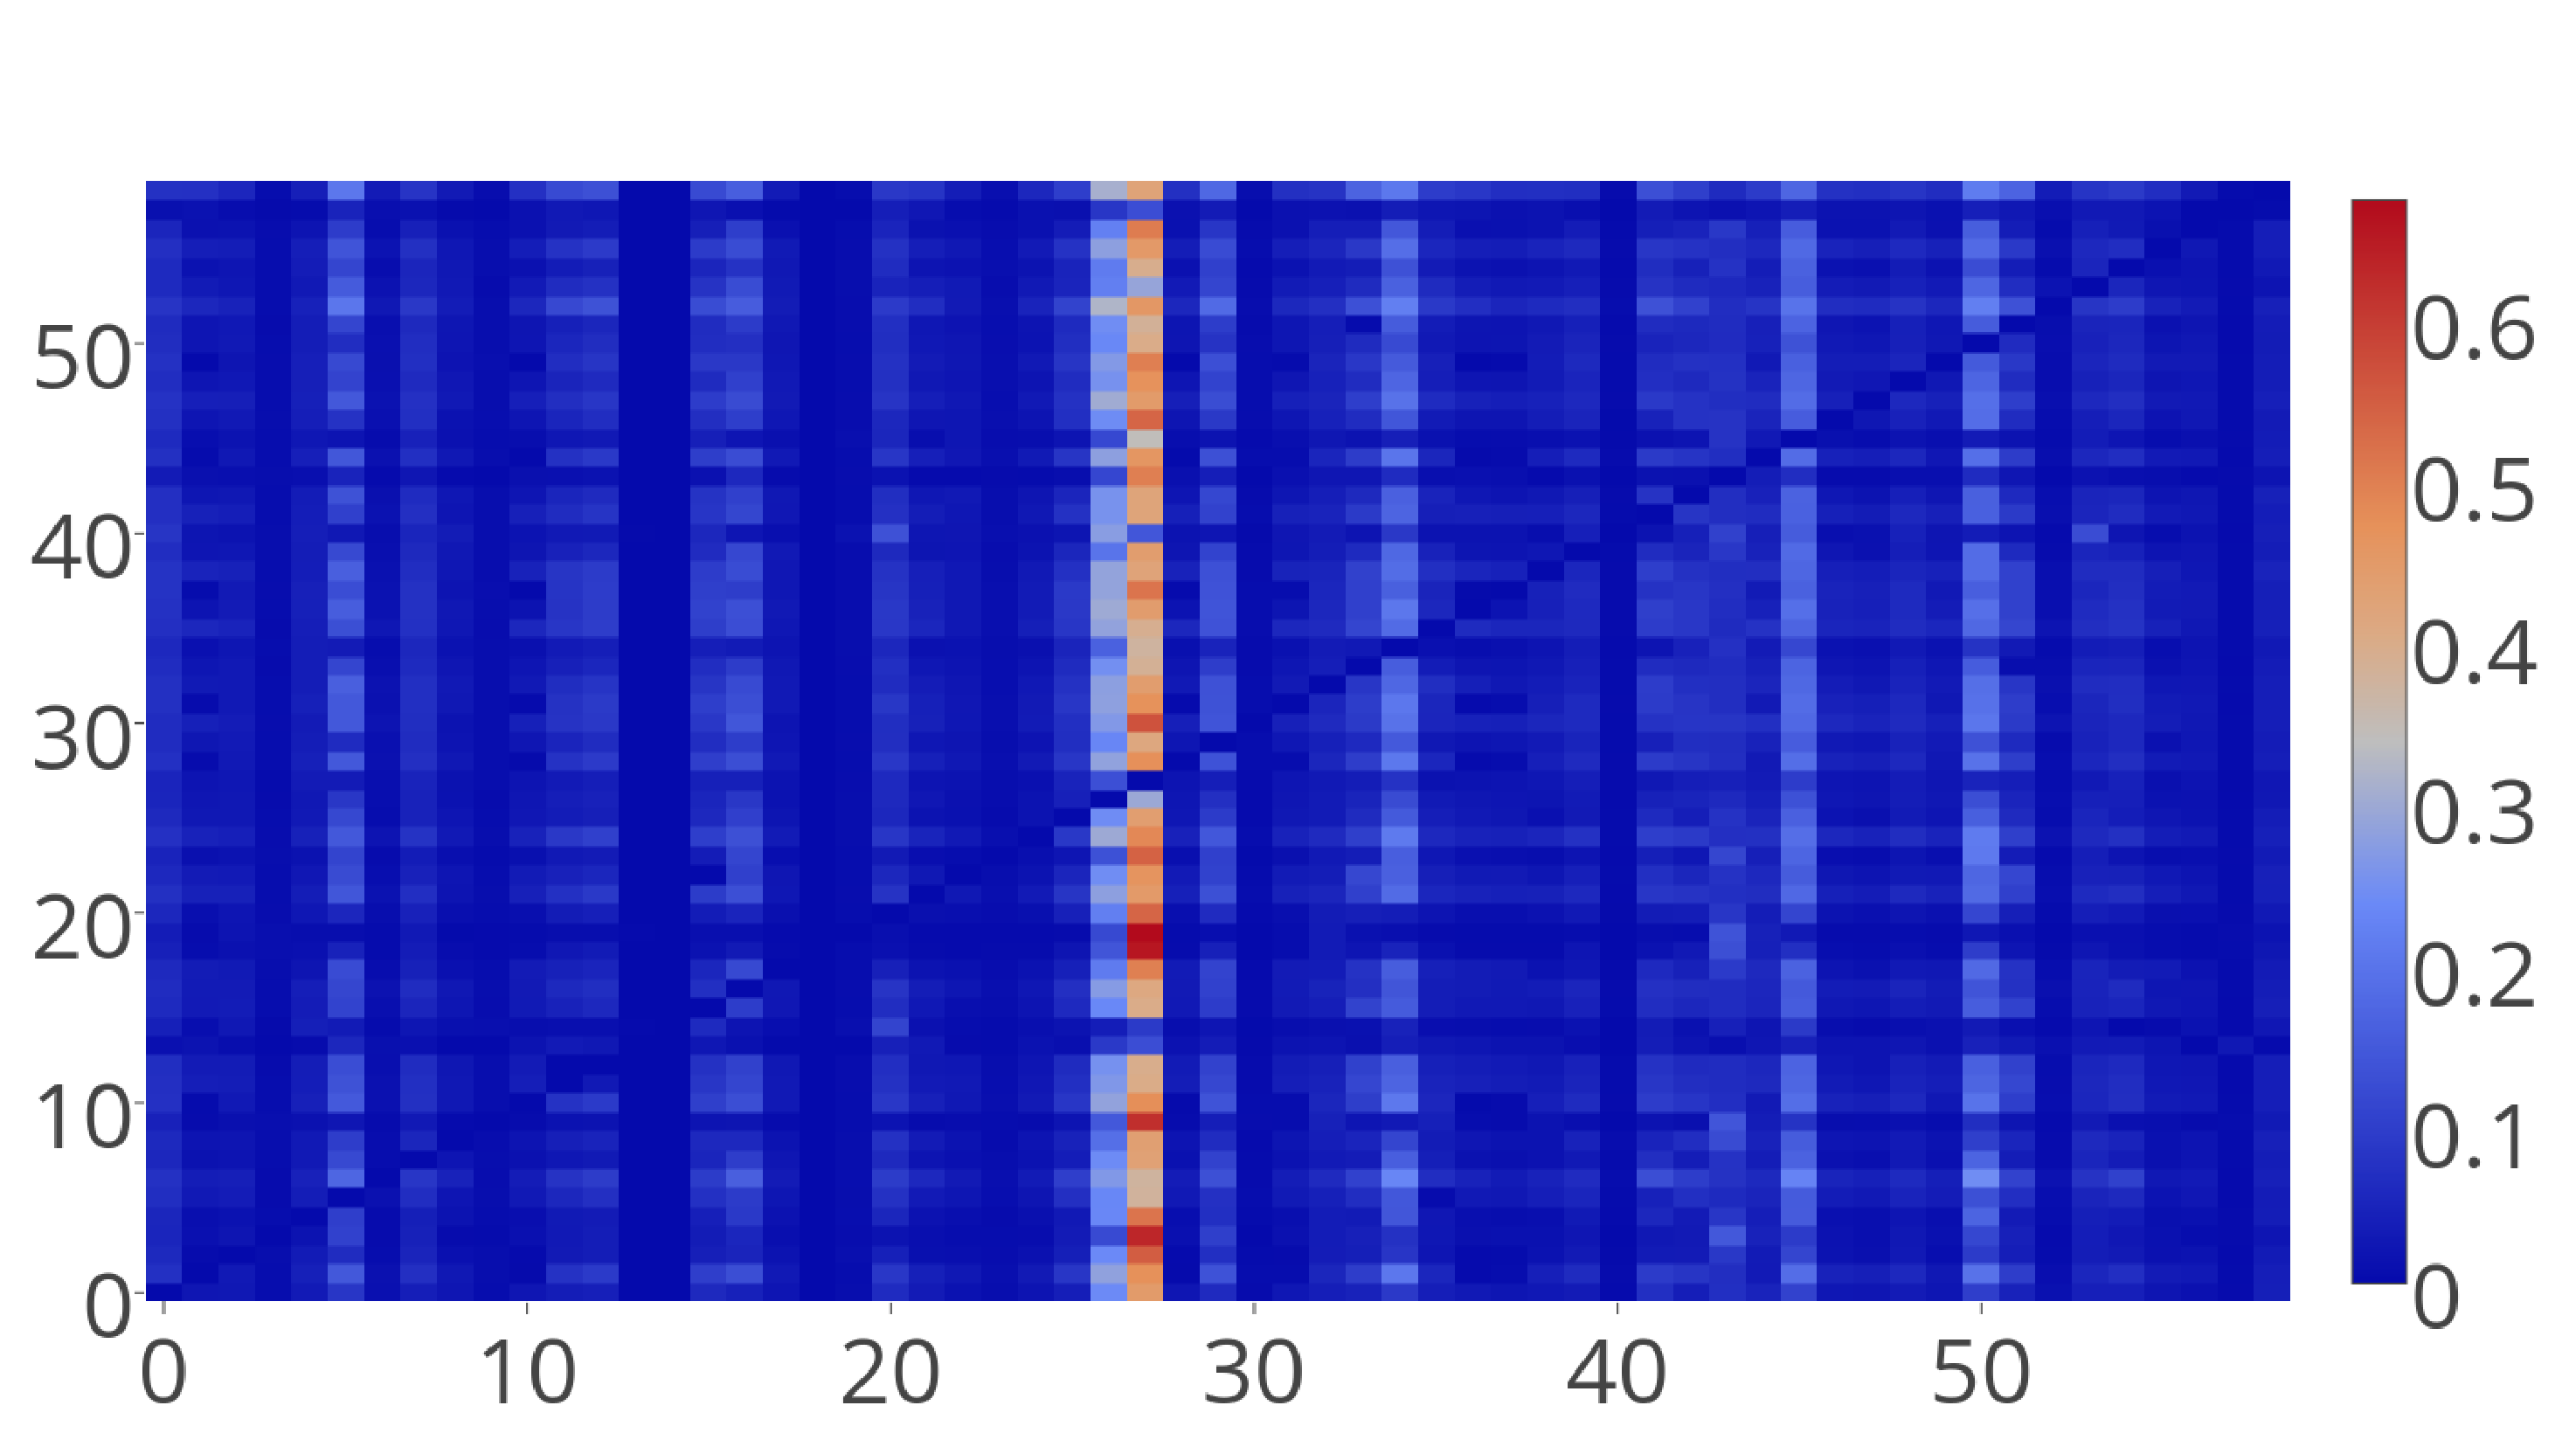
\includegraphics[width=0.24\linewidth]{figure/bernoulli-train}\label{fig:moredata1}} 
\subfloat[]{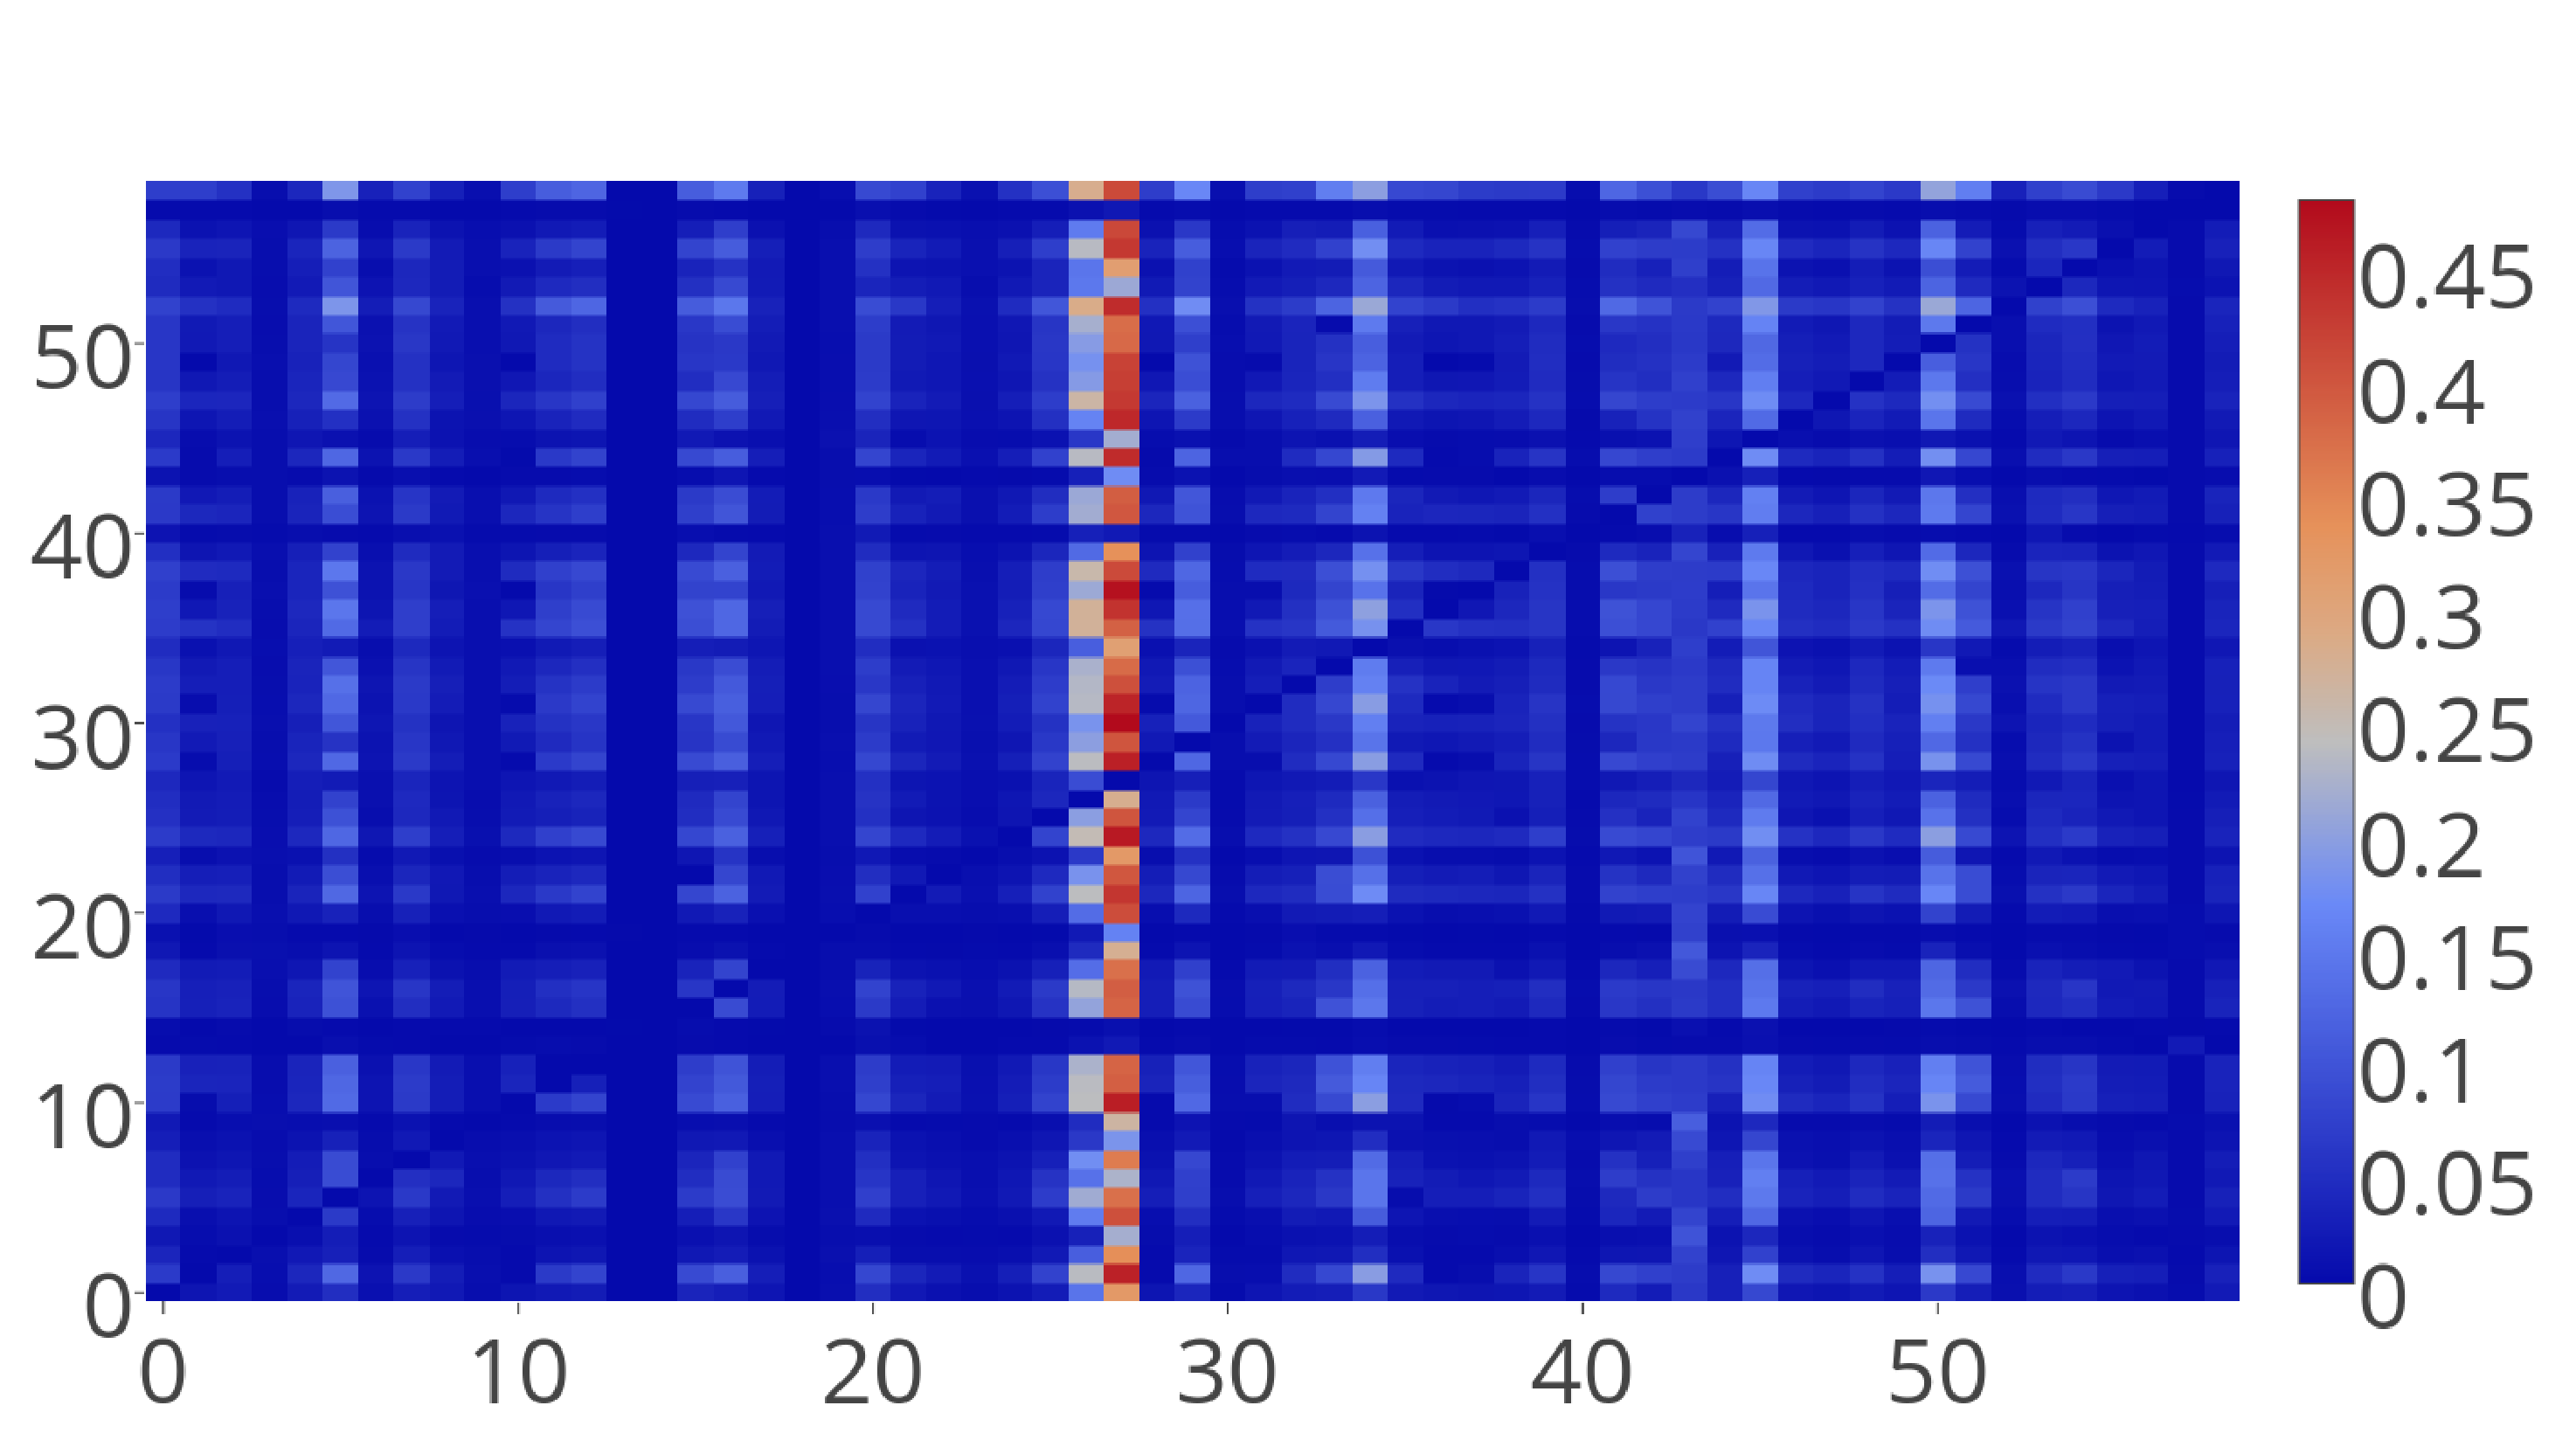
\includegraphics[width=0.24\linewidth]{figure/jaccard-train}\label{fig:moredata2}}
\subfloat[]{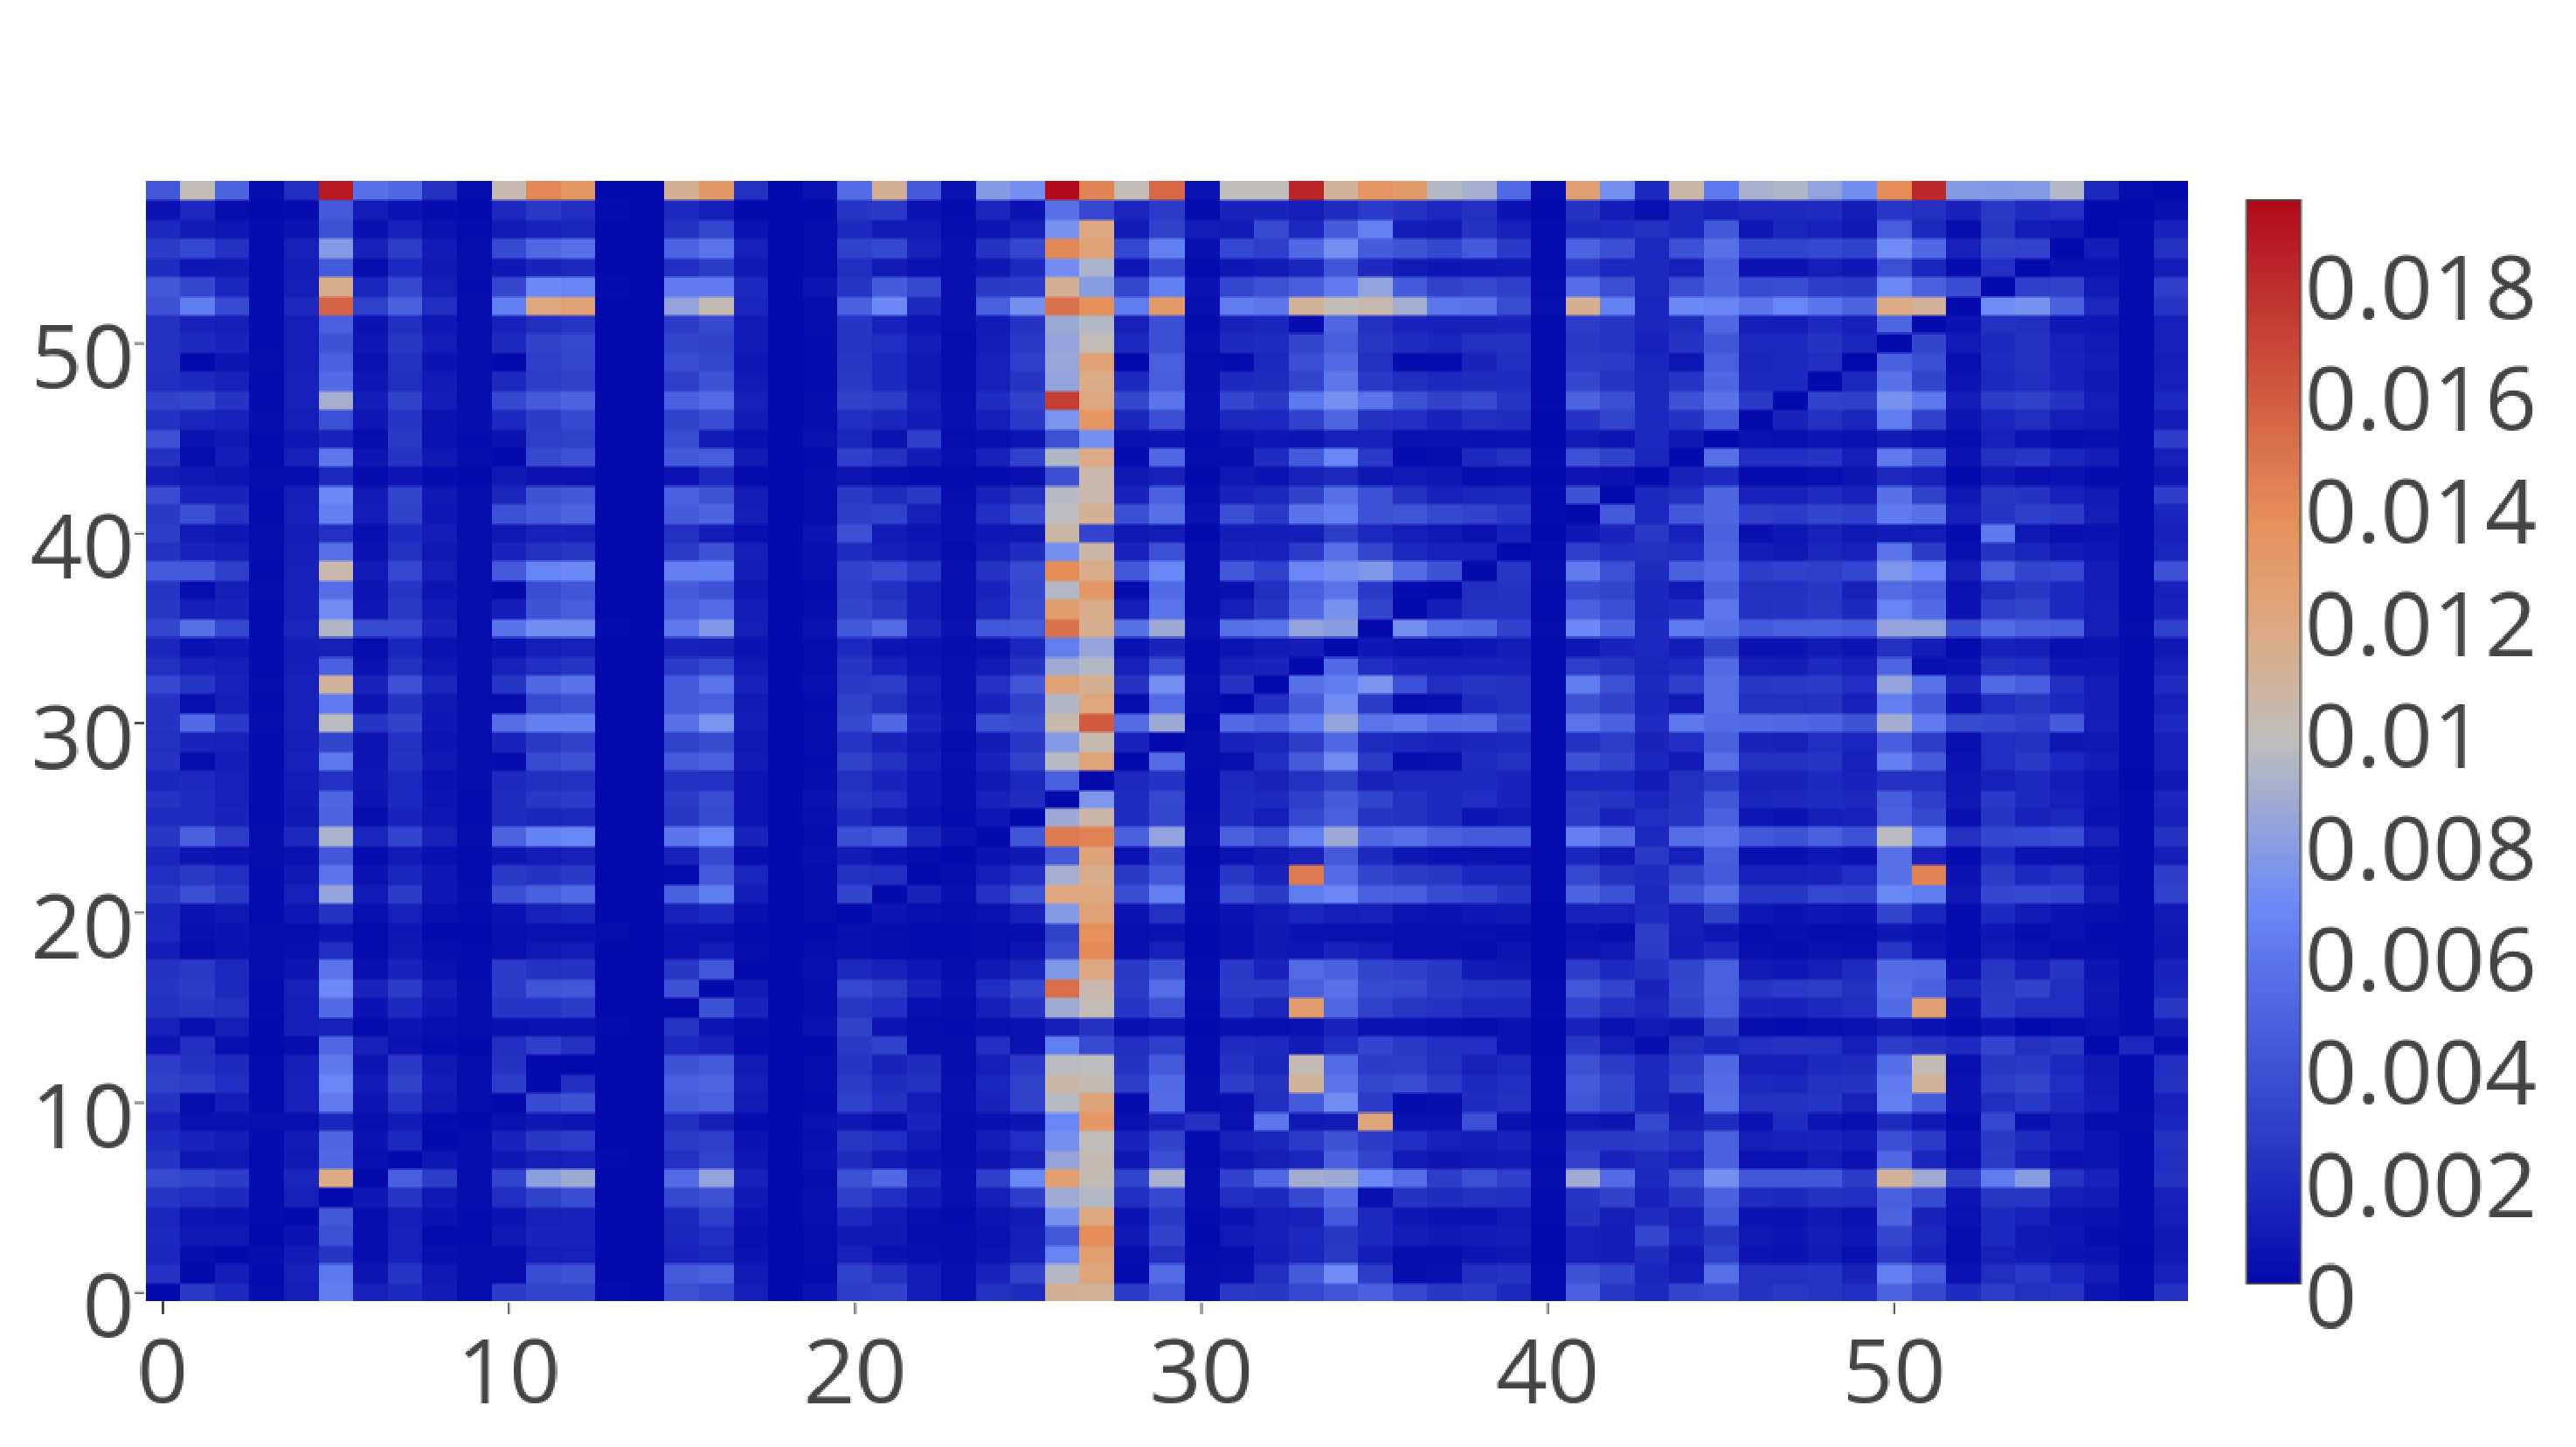
\includegraphics[width=0.24\linewidth]{figure/PC-train}\label{fig:moredata3}} 
\subfloat[]{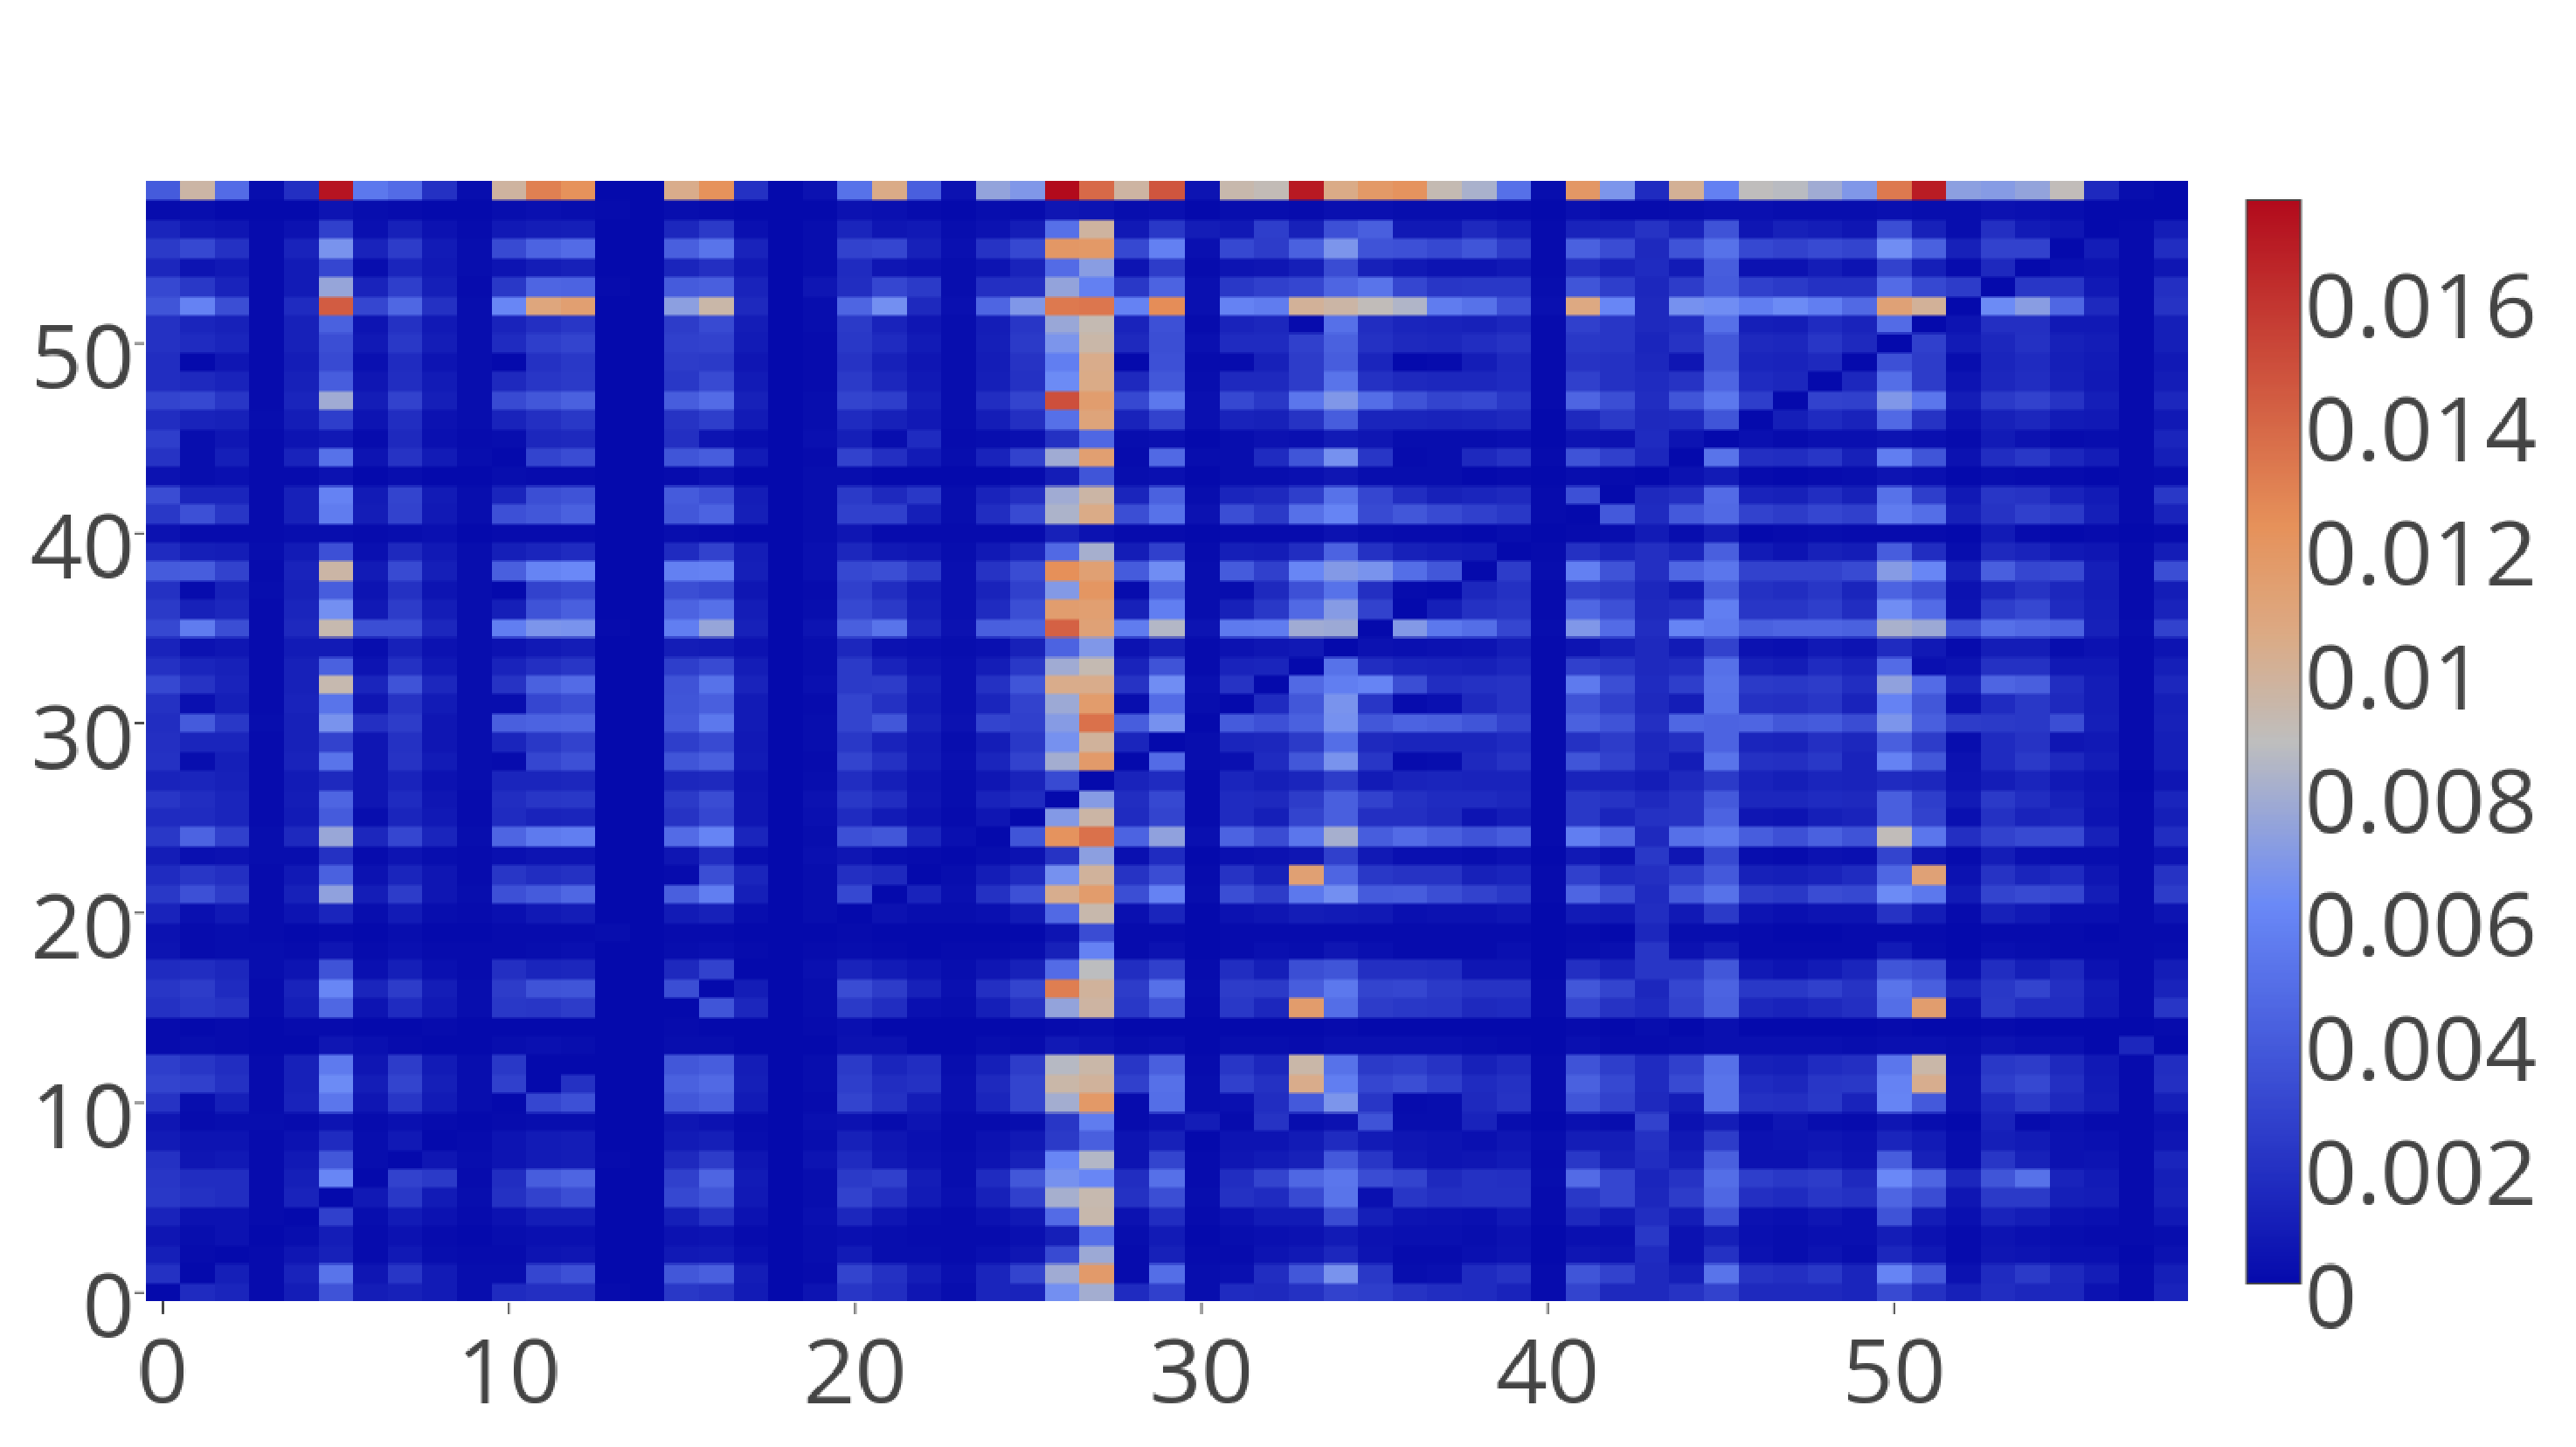
\includegraphics[width=0.24\linewidth]{figure/jaccardPC-train}\label{fig:moredata4}} \\ 
\caption{Potential for 0.5 V bias.} 
\label{fig:EcUND} 
\end{figure*} 


\begin{figure}[t!]
\begin{center}
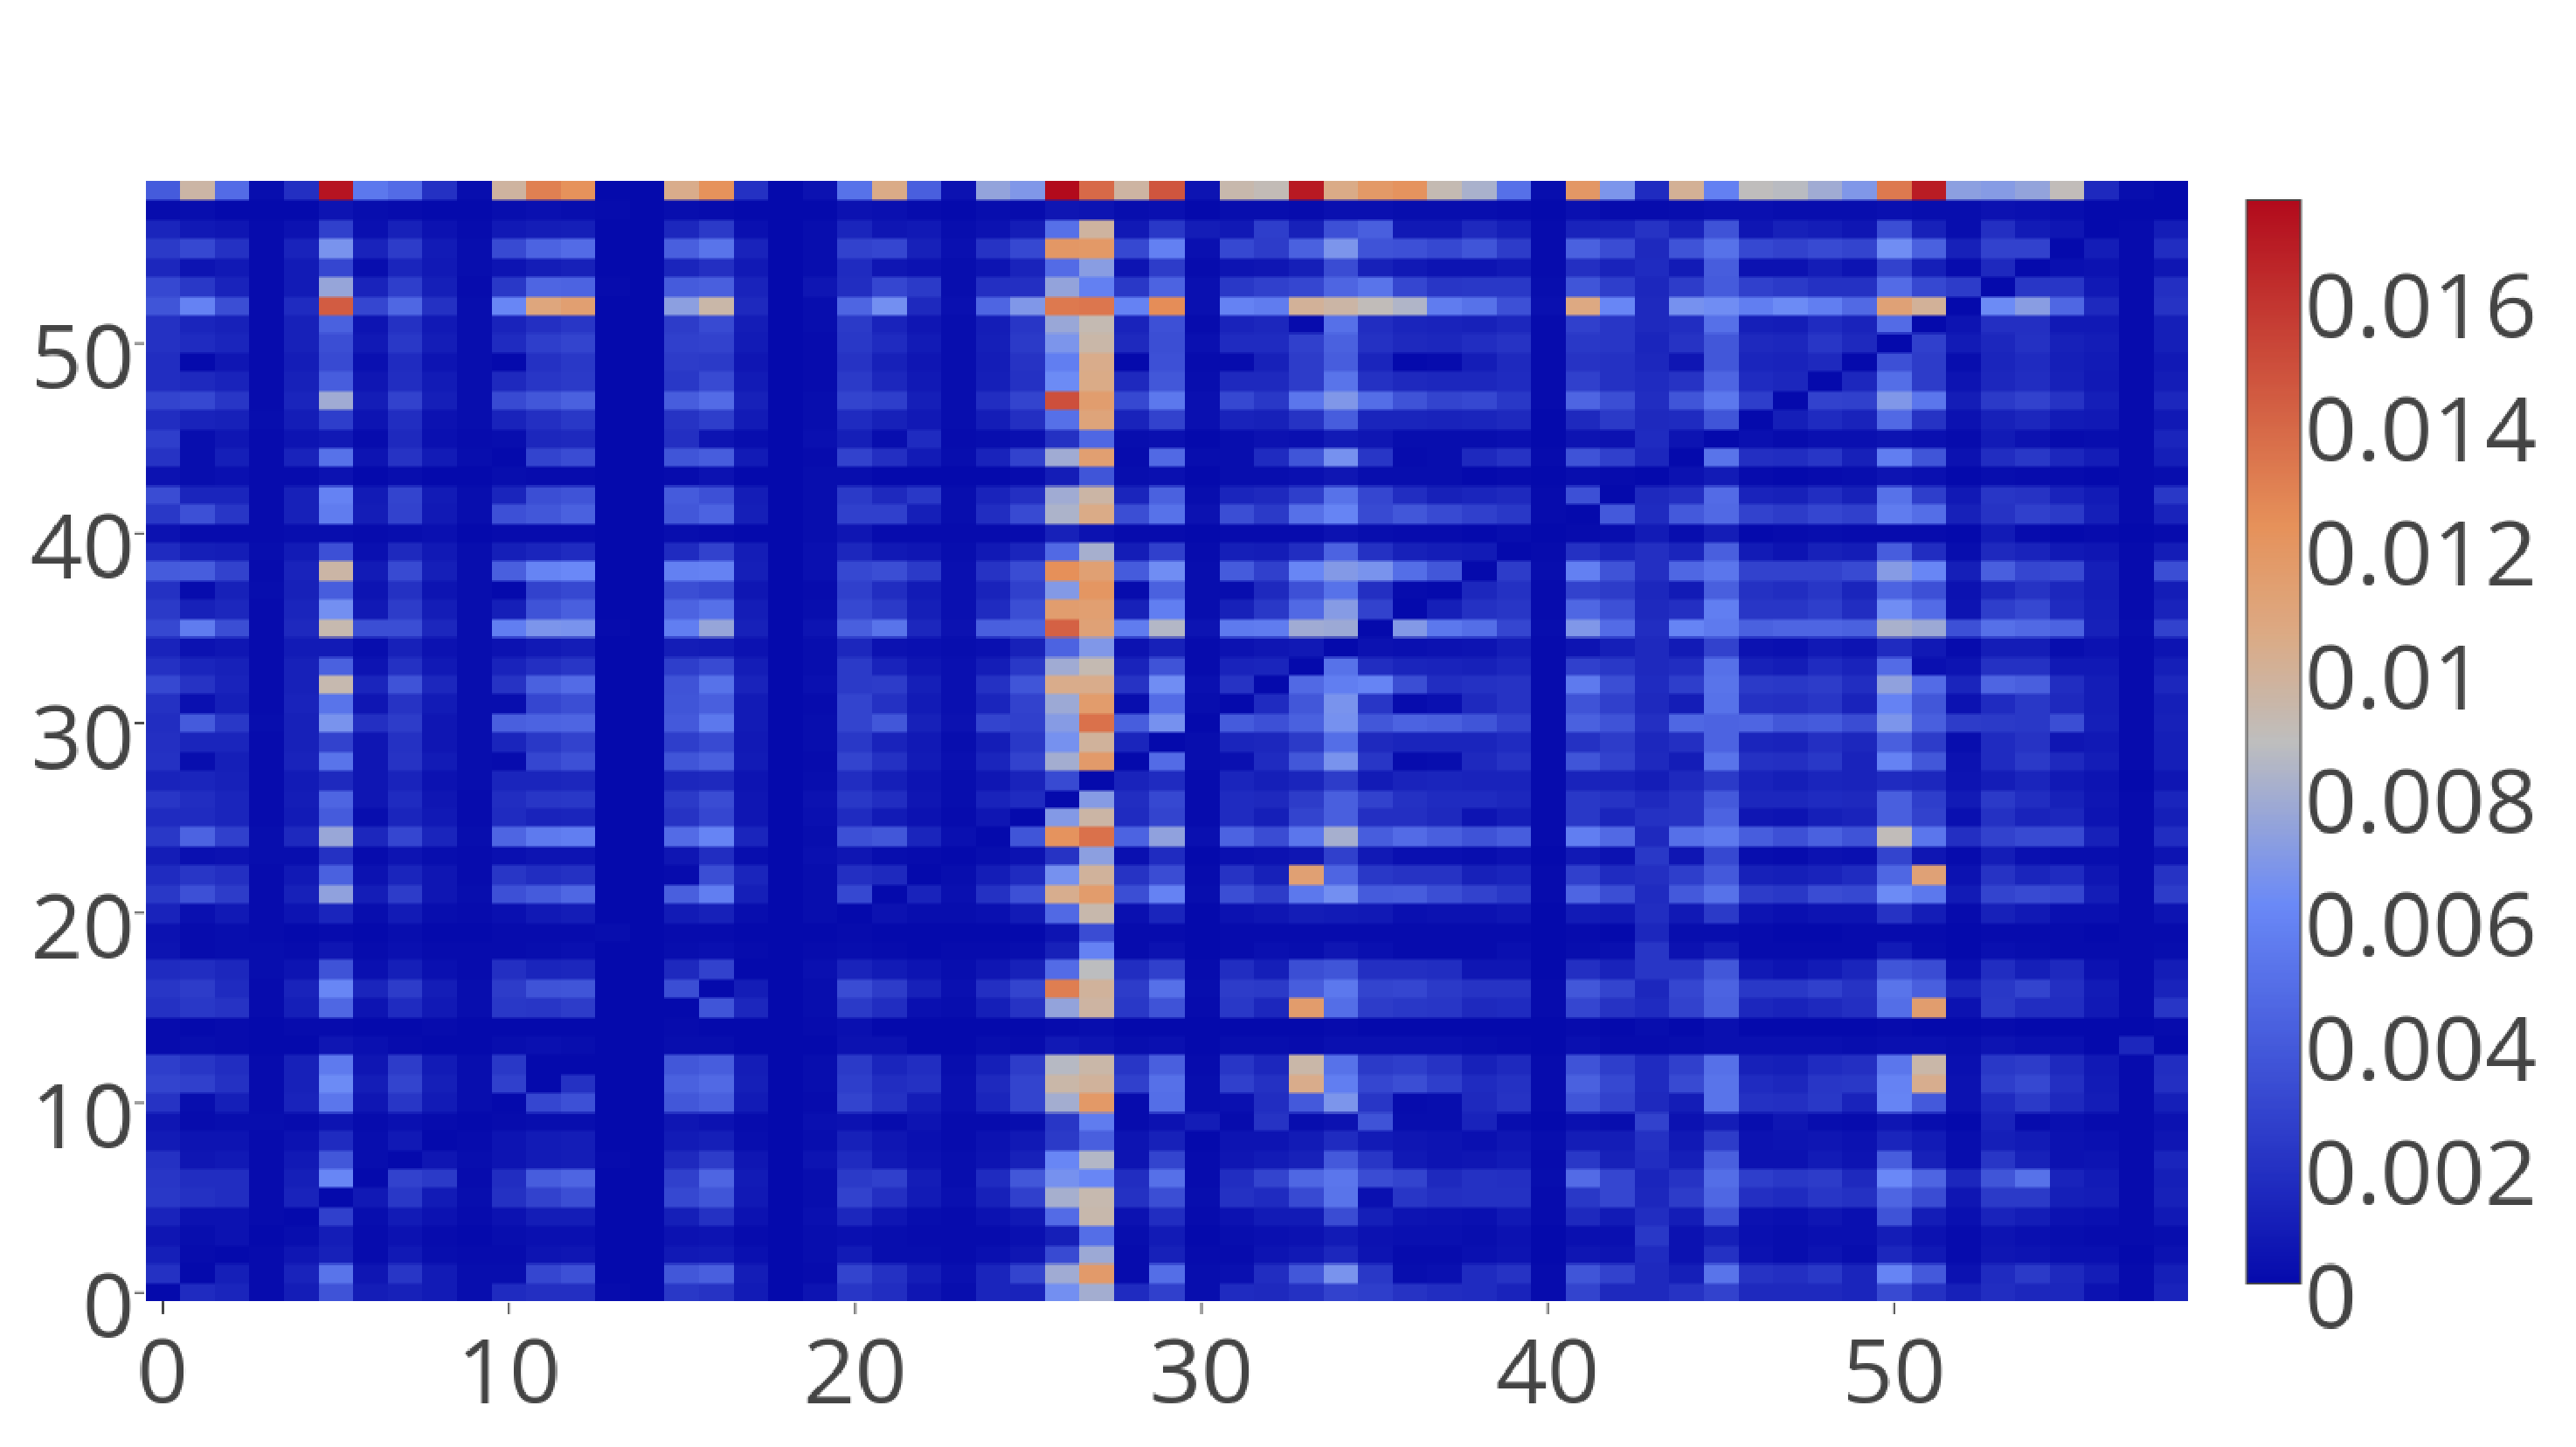
\includegraphics[width=2.5in]{figure/jaccardPC-train}
\mycaption{fig:idreputation}{Test.}
{\footnotesize{(How detection rate changes with the value of source id's reputation. Each reputation is rounded up to nearest 0.05.
Reputation -1 means the source id did not make any submission before. 95\% confidence interval is also drawn 
for each point.)}}
\end{center}
%\vspace{-0.25in}
\end{figure}


\subsection{Influence Probability Analysis}
\label{sec:influenceanalysis}

Using the four static models discussed above, we built an influence graph with anti-virus engines on \vt\ and analyzed 
the influence probability ($p_{u,v}$) between each pair of engines.

\noindent{\underline{\textit{Methodology.}}}
We implement our analysis using several stages of map, filter, and reduce in Spark~\cite{spark}. 
Specifically, we first map submission records according to their corresponding files
and filter out submissions without action propagation. 

\if 0
{\color{red} XXX I don't get the following paragraph. Do we really need this much impl details?}
We then sort submission records for each remaining submitted file chronologically in a map stage.
In the next map stage, we compute four hash tables for each submitted file based on all its submissions.   
There is one one-dimension hash table, containing whether the action to identify the submitted file as malware is taken by each vendor ($|A_{u}|$). 
There are three two-dimension hash tables, 
containing an entry for each pair of vendors $(u,v)$, 
representing whether both $u$ and $v$ take the action ($|A_{u\&v}|$),  
whether the action is propagated from $u$ to $v$ ($|A_{u2v}|$),
and partial credit taken by $u$ if the action is propagated from $u$ to $v$ ($credit_{u,v}(a)$).
After this stage, $|A_{u}|$, $|A_{u\&v}|$, and $|A_{u2v}|$ are either 0 or 1,
and $credit_{u,v}(a)$ is 0 or not larger than 1, since all these values are calculated for one single submitted file. 
In the final stage, 
we reduce these 4 hash tables from different files,
and calculate $p_{u,v}$ for the four static models. 
\fi

We then filter out engines taking fewer than 20000 actions,
since engines taking too few actions cannot produce meaningful results.
There are 59 engines left,
and the average number of actions taken by these engines is around 392K. %190140, which is much larger than 10000.
For confidentiality reasons, we omit vendors' name in the following discussion
and use numbers from 0 to 58 to represent these vendors.

\noindent{\underline{\textit{Analysis results and implications.}}}
For each static model, 
we construct an influence table with calculated influence probability values ($p_{u,v}$), 
with $u$ as row number and $v$ as column number.
We visualize these influence tables with heat maps in Figure~\ref{fig:heat}. 
Each $cell(u, v)$ represents the relative heat color of $p_{u,v}$, 
and red means more influence from $u$ to $v$. 

We also sum all $p_{u,v}$ values in a column in each influence table 
to calculate trustworthiness of engine $v$ using Equation~\ref{eq:trust}. 
Table~\ref{tab:trust} lists the maximum, minimum, and average trustworthiness values of all the engines under four different models.
The results can serve as a quantitative measurement for how trustworthy anti-virus engines are. 

In all the four heat maps, there are two columns with almost all cells in red,
which means that these vendors influenced by all other vendors and are less trustworthy.
On the other hand, quite a few vendors are not influenced by any vendors (blue columns).
This result suggests that most vendors perform predictions on their own and thus can be trusted. 
However, our result should also ring an alarm to online malware detection service users and security experts that 
we cannot treat all engines with the same level of trust 
and the results from some of them should be at least examined more closely if not discarded.

At the same time, there are several rows with many cells in red, especially in the last two heat map, 
which means that there are vendors which influence many vendors,
where there are a set of vendors that do not influence other vendors (blue rows).
Different from the effect of columns which shows the trustworthiness of a vendor by users, 
the effect of rows is related to how vendors view (and trust) each other. 
Certain vendors are highly regarded by many other vendors so that 
their decision results are often referenced by other vendors.

Interestingly, the vendors that are heavily influenced by others are not the ones that influence others, 
suggesting that the vendors with lower trustworthiness by users are also not trusted by other vendors. 

\begin{table}[h!]
\centering
\footnotesize
{
\begin{tabular}{l|l|l|l}
\hline
Model                & Max     & Min & Average \\
\hline                            
%\cline{1-1}
{\bf Bernoulli}                    & 108.78   & 0.04 & 5.40 \\
{\bf Jaccard Index}                & 118.20   & 0.05 & 6.15 \\
{\bf Bernoulli with Partial Credit} & 3545.34  & 1.63 & 138.45 \\
{\bf Jaccard Index with Partial Credit} & 4177.98 & 2.02 & 155.18 \\
\hline
\end{tabular}
}
\caption{Trustworthiness. 
%\footnotesize{
(Maximum, minimum, and average trustworthiness values under four different models.)
%}
}
\label{tab:trust}
\end{table}


Finally, we observe that although the four static models show similar trends of influence relationship 
and the relative rankings of engines in terms of influence are similar,
their absolute influence probability values differ. 
Bernoulli distribution and Jaccard index have influence probability values
that are about 30 to 40 times higher than
Bernoulli and Jaccard index with partial credit. 
%This shows that {\color{red} influence is shared among vendors take actions earlier than others. I have no idea what sentense means. if you cannot explain well, just remove this sentence.}.

{\bf Observation 8:} 
{\em Certain anti-virus vendors are influenced by almost all other vendors in their malware detection decisions and are less trustworthy, 
while quite a few trustworthy vendors have influence on many other vendors.}

\subsection{Influence Probability Prediction}
\label{sec:predict}

The analysis results of vendor influence above are encouraging.
With these results, we take a step further and ask 
{\em if it is possible to predict whether or not an engine's prediction of 
a file submission should be trusted (i.e., not influenced by other engines)?}
We now discuss the prediction model we built to answer this question.

\noindent{\underline{\textit{Methodology.}}}
We first split all the \pe\ submissions we collected into a training set and a testing set based on 
the SHA256 values of the submitted files. 
We place all submissions with SHA256 values starting with a numeric character, 
i.e., from `0' to `9', into training set
and all the rest (starting from 'a' to 'f') into the testing set.
We use Spark to implement both the training and the testing process.
%Similar to our training stage process, 
%we first reduce all submissions based on submitted files,
%next filter out files without action propagation, 
%and then sort submissions chronologically. 


%\noindent{\underline{\textit{Training stage methodology.}}}
During the training stage, we use the training set to build an influence graph and
learn $p_{u,v}$ of each edge in the graph using the four static models discussed in Section~\ref{sec:influenceprob}.
The calculation of $p_{u,v}$ is the same as in Section~\ref{sec:influenceanalysis}.

%\noindent{\underline{\textit{Testing stage methodology.}}}
During the prediction stage, for each submission in the testing set, 
we predict whether or not an engine $v$ will take an action $a$ following other engines 
if it has not taken that action yet. 
%Specifically, we use a tunable threshold $\theta$
%and predict $v$ will follow its neighbors to take the action $a$ in the future
%if $p_v(S_v(a))>\theta$.
Specifically, to test a submission, we first use Equation~\ref{eq:setp} to
calculate $p_v(S_v(a))$, the probability that $v$ will follow its neighbors to take the same action, 
for all engines that have labeled the submitted file only as benign in their history. 
These engines are of interest to us because positive influence, 
the type of influence in this study, only happens 
when an engine changes its prediction decision from benign to malware.

We then compare $p_v(S_v(a))$ with a {\em tunable threshold $\theta$} to predict whether $v$ will label the file as malware (if $p_v(S_v(a))>\theta$) or not.
Next, we compare this prediction with the actual action that $v$ took in the testing set to deduct true positives (TPs) where both our prediction 
and the actual fact label the submission as malware, 
false negatives (FNs) where our prediction labels the submission as benign and the actual labeling is malware. 
Thus, TP means our prediction is the same as the fact 
and both show the engine changes its labeling from benign to malware, an indication that the decision 
of this engine on the submission is in deed affected by other engines.
Similarly, we can obtain false positives (FPs) 
and true negatives (TNs).
%After processing all submissions for a file, 
%we calculate $p_v(S_v(a))$ for all engines  
%that label the file as benign but have not labeled the file as malware.
%We compare $p_v(S_v(a))$ with $\theta$ to count false positives (FPs) and true negatives (TNs).
In the final stage, we calculate the overall TP, TN, FP, and FN rates for all different files.

\begin{figure}[t!]
\begin{center}
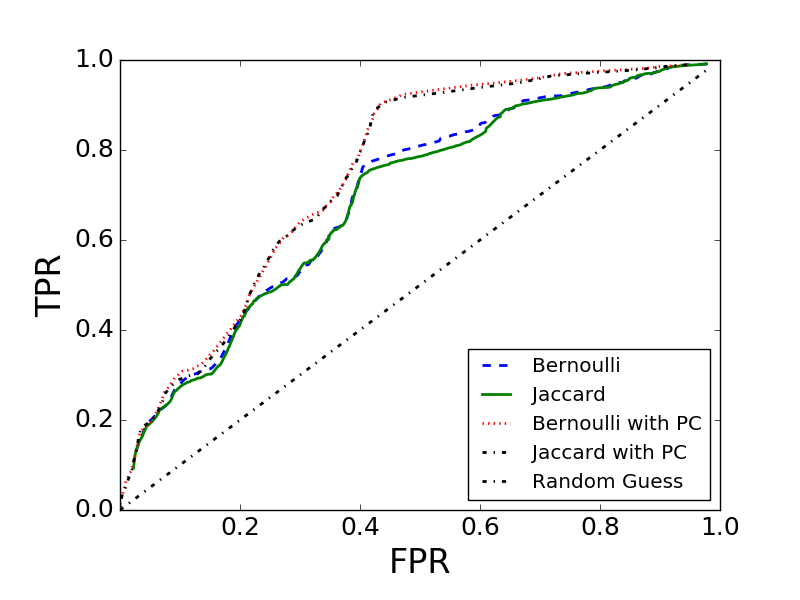
\includegraphics[width=2in]{figure/predict}
\vspace{-0.1in}
\caption{ROC comparisons of Static Models. 
(How true positive rate (TPR) changes with false positive rate (FPR). 
We change probability threshold from 0.1\% to 99.9\% with step 0.1\%. 
We compute TPR and FPR for each probability threshold to draw the curve.)
}
\label{fig:predict}
\end{center}
\vspace{-0.1in}
\end{figure}

\noindent{\underline{\textit{Prediction results.}}}
We change the threshold $\theta$ from 0.1\% to 99.9\% 
and measure the accuracy of the four static models using ROC (Receiver Operating Characteristic) curves,
with true positive rate ($TPR = TP/(TP+FN)$) as X-axis
and false positive rate ($FPR = FP/(FP + FN)$) as Y-axis. 
Figure~\ref{fig:predict} plots the ROC curves for the four static models.
A larger area under the ROC curve means higher accuracy.
We compare our prediction models with random guess, 
which is represented by the diagonal line between (0,0) to (1,1) in the figure. 

We find that all models are more accurate than random guess
and using partial credits improves the accuracy of both Bernoulli and Jaccard index.
This result is encouraging;
even with a simple prediction model like ours, we can already obtain satisfactory prediction accuracy of whether an engine's decision has been influenced by others.

{\bf Observation 9:} 
{\em Our influence prediction model can accurately predict whether or not an anti-virus engine's labeling of a submission should be trusted. }

\subsection{Discussion}
%Our scientific analysis on vendor influence in this section confirms our XXX
Our findings in this section shed light on how vendors can influence each other and rings an alert towards using detection rate as the only measurement of the likelihood of a file being malware.
Our study results can serve as a quantitative measurement for vendors' influence in malware detection community. 
Previously, when combining results from different vendors, 
security experts simply treat each vendor equally and use the percentage of 
vendors labeling a file as malware as likelihood of the file to be a malware. 
Our model can provide a weight to each vendor 
when combining results from different vendors.  
Anti-virus vendors can also use our prediction model to detect possible false negatives in their products.

\if 0
{\color{red} Do we really need this (the following two paragraphs)? this sounds very defensive}
%\if 0
There are also time models proposed by~\citet{Influence}.
When analyzing Flickr data, time models leverage accurate action time to provide better prediction performance. 
However, we do not use time models, 
because time information we access is when a submission is conducted, 
or when an engine analyzes a submission, 
is not when an engine changes its detection label for a file.
The time information we have can only provide a relative order about when each vendor identifies a file as malware.  

%\underline{Limitation.}
Our data collection ends on September 6th, 2016. 
We could count extra FPs, where we predict engines will label files as malware, engines have not, but will do in the future, 
and TNs, where we predict engine will not label, engines have not, but will in the future. 
Monitoring \vt for a longer time will make the evaluation of our prediction models more precise. 

%\underline{How to use?}
\fi


\section{Prediction Model}

\subsection{Overview}

What do we want to predict?

a. Whether a file is stable now

b. decision tree

\subsection{Experiments and implications}


\section{Related works}

The AISec Paper

\section{Conclusions}


%\section{Introduction}

This is a sample!  It does not have a lot of fancy stuff in it, but if
you want to see a more complex sample, look at the original ACM
templates.

To fill up enough text to fill up 3 pages, we've included the CCS Call
for Papers three times.  It is always a good idea to include some
gratuitious citations to recent CCS papers~\cite{medvinsky1993netcash,
  bellare1993random, anderson1993cryptosystems, blaze1993cryptographic}.

\section{Call for Papers}

The conference seeks submissions presenting novel research results in
all aspects of computer and communications security and privacy,
including both practical and theoretical contributions.

\subsection{Paper Submission Information}

Submissions must be received at \url{https://ccs17.hotcrp.com/} by the
strict deadline of {\bf 19 May 2017 at 8:59 PM PDT (UTC-7)}.
Submitted papers must not substantially overlap with papers that have
been published or that are simultaneously submitted to a journal,
conference, or workshop. Submissions must be anonymized and avoid
obvious self-references.

CCS has traditionally required that authors submitting papers
guarantee that an author will be able to present their paper at the
conference. We recognize, however, that the current travel
restrictions and screening processes may make it impossible or
uncomfortable for some authors to travel to the conference. The venue
for CCS 2017 was selected several years ago, and we do not wish to
exclude any potential authors who may have difficulty traveling due to
recent changes in US immigration practices.  CCS welcomes submissions
by authors of all nationalities, and will make allowances for
presenting papers electronically or with non-author presenters in
cases where paper authors are unable to travel to the United States.

Submissions will be evaluated based on their scientific merit,
novelty, importance, presentation quality, and relevance to computer
and communications security and privacy.  If a paper includes work
that raises ethical concerns it is up to the authors to convince the
reviewers that appropriate practices were followed to minimize
possible harm and that any harm caused by the work is greatly
outweighed by its benefits. The review process will be carried out in
two phases and authors will have an opportunity to provide a
length-limited response to the first-phase reviews.

\subsection{Paper Format}

Submissions must be single PDF files containing at most 12 pages in
the required new ACM format (see
\url{https://www.sigsac.org/ccs2017/format} for details and templates,
which you have presumably found if you are reading this!) of body
content, with any number of additional pages for the bibliography,
well-marked appendices, and any desired supplementary material.  When
relevant, submitters may include reviews from past submissions and
responses to them in the supplementary material.

Reviewers are not required to consider the appendices or supplementary
material, however, so submissions need to be intelligible and
convincing without them.  Submissions not meeting these guidelines, or
playing games to work around page limits, will be rejected by the PC
chairs without review.  In particular, papers should not use squeezing
tricks to adjust the (already very dense) ACM paper format, and moving
discussion of key related work or important definitions to appendices
may be grounds for rejection.

\subsection{Practice Talks}

Following the lead of USENIX Enigma, we want to improve the quality of
the conference and provide a better experience for both presenters and
attendees by holding practice sessions before the conference (see
\url{https://www.sigsac.org/ccs2017/practicefaq}). Presenting authors
of accepted papers are expected to participate in an on-line practice
session approximately three weeks before the conference.

\subsection{Conflicts of Interest}

The conference requires cooperation from both authors and program
committee members to ensure a process that is both fair in practice
and perceived to be fair by everyone. When submitting a paper, authors
are required to identify members of the program committee who may not
be able to provide an unbiased review.  This includes people with
strong personal or professional relationships such as advisor/advisee,
members of the same organization, and close collaborators (for
example, recent or repeated co-authors). In general, this means anyone
who a reasonable person with all the relevant information would
question as an impartial reviewer. The program co-chairs reserve the
right to request a more specific description of a conflict-of-interest
declaration from authors.

Program committee members who have a conflict of interest with a
paper, including program co-chairs, will be excluded from evaluation
and discussion of the paper, but because submissions are anonymous to
reviewers it is important for submitting authors to identify these
conflicts. In the case of a program co-chair, the other co-chairs who
do not have conflicts will be responsible for managing that paper.
Program co-chairs are not permitted to be involved as co-authors in
any submissions.



\section{Call for Papers}

The conference seeks submissions presenting novel research results in
all aspects of computer and communications security and privacy,
including both practical and theoretical contributions.

\subsection{Paper Submission Information}

Submissions must be received at \url{https://ccs17.hotcrp.com/} by the
strict deadline of {\bf 19 May 2017 at 8:59 PM PDT (UTC-7)}.
Submitted papers must not substantially overlap with papers that have
been published or that are simultaneously submitted to a journal,
conference, or workshop. Submissions must be anonymized and avoid
obvious self-references.

CCS has traditionally required that authors submitting papers
guarantee that an author will be able to present their paper at the
conference. We recognize, however, that the current travel
restrictions and screening processes may make it impossible or
uncomfortable for some authors to travel to the conference. The venue
for CCS 2017 was selected several years ago, and we do not wish to
exclude any potential authors who may have difficulty traveling due to
recent changes in US immigration practices.  CCS welcomes submissions
by authors of all nationalities, and will make allowances for
presenting papers electronically or with non-author presenters in
cases where paper authors are unable to travel to the United States.

Submissions will be evaluated based on their scientific merit,
novelty, importance, presentation quality, and relevance to computer
and communications security and privacy.  If a paper includes work
that raises ethical concerns it is up to the authors to convince the
reviewers that appropriate practices were followed to minimize
possible harm and that any harm caused by the work is greatly
outweighed by its benefits. The review process will be carried out in
two phases and authors will have an opportunity to provide a
length-limited response to the first-phase reviews.

\subsection{Paper Format}

Submissions must be single PDF files containing at most 12 pages in
the required new ACM format (see
\url{https://www.sigsac.org/ccs2017/format} for details and templates,
which you have presumably found if you are reading this!) of body
content, with any number of additional pages for the bibliography,
well-marked appendices, and any desired supplementary material.  When
relevant, submitters may include reviews from past submissions and
responses to them in the supplementary material.

Reviewers are not required to consider the appendices or supplementary
material, however, so submissions need to be intelligible and
convincing without them.  Submissions not meeting these guidelines, or
playing games to work around page limits, will be rejected by the PC
chairs without review.  In particular, papers should not use squeezing
tricks to adjust the (already very dense) ACM paper format, and moving
discussion of key related work or important definitions to appendices
may be grounds for rejection.

\subsection{Practice Talks}

Following the lead of USENIX Enigma, we want to improve the quality of
the conference and provide a better experience for both presenters and
attendees by holding practice sessions before the conference (see
\url{https://www.sigsac.org/ccs2017/practicefaq}). Presenting authors
of accepted papers are expected to participate in an on-line practice
session approximately three weeks before the conference.

\subsection{Conflicts of Interest}

The conference requires cooperation from both authors and program
committee members to ensure a process that is both fair in practice
and perceived to be fair by everyone. When submitting a paper, authors
are required to identify members of the program committee who may not
be able to provide an unbiased review.  This includes people with
strong personal or professional relationships such as advisor/advisee,
members of the same organization, and close collaborators (for
example, recent or repeated co-authors). In general, this means anyone
who a reasonable person with all the relevant information would
question as an impartial reviewer. The program co-chairs reserve the
right to request a more specific description of a conflict-of-interest
declaration from authors.

Program committee members who have a conflict of interest with a
paper, including program co-chairs, will be excluded from evaluation
and discussion of the paper, but because submissions are anonymous to
reviewers it is important for submitting authors to identify these
conflicts. In the case of a program co-chair, the other co-chairs who
do not have conflicts will be responsible for managing that paper.
Program co-chairs are not permitted to be involved as co-authors in
any submissions.



\section{Call for Papers}

The conference seeks submissions presenting novel research results in
all aspects of computer and communications security and privacy,
including both practical and theoretical contributions.

\subsection{Paper Submission Information}

Submissions must be received at \url{https://ccs17.hotcrp.com/} by the
strict deadline of {\bf 19 May 2017 at 8:59 PM PDT (UTC-7)}.
Submitted papers must not substantially overlap with papers that have
been published or that are simultaneously submitted to a journal,
conference, or workshop. Submissions must be anonymized and avoid
obvious self-references.

CCS has traditionally required that authors submitting papers
guarantee that an author will be able to present their paper at the
conference. We recognize, however, that the current travel
restrictions and screening processes may make it impossible or
uncomfortable for some authors to travel to the conference. The venue
for CCS 2017 was selected several years ago, and we do not wish to
exclude any potential authors who may have difficulty traveling due to
recent changes in US immigration practices.  CCS welcomes submissions
by authors of all nationalities, and will make allowances for
presenting papers electronically or with non-author presenters in
cases where paper authors are unable to travel to the United States.

Submissions will be evaluated based on their scientific merit,
novelty, importance, presentation quality, and relevance to computer
and communications security and privacy.  If a paper includes work
that raises ethical concerns it is up to the authors to convince the
reviewers that appropriate practices were followed to minimize
possible harm and that any harm caused by the work is greatly
outweighed by its benefits. The review process will be carried out in
two phases and authors will have an opportunity to provide a
length-limited response to the first-phase reviews.

\subsection{Paper Format}

Submissions must be single PDF files containing at most 12 pages in
the required new ACM format (see
\url{https://www.sigsac.org/ccs2017/format} for details and templates,
which you have presumably found if you are reading this!) of body
content, with any number of additional pages for the bibliography,
well-marked appendices, and any desired supplementary material.  When
relevant, submitters may include reviews from past submissions and
responses to them in the supplementary material.

Reviewers are not required to consider the appendices or supplementary
material, however, so submissions need to be intelligible and
convincing without them.  Submissions not meeting these guidelines, or
playing games to work around page limits, will be rejected by the PC
chairs without review.  In particular, papers should not use squeezing
tricks to adjust the (already very dense) ACM paper format, and moving
discussion of key related work or important definitions to appendices
may be grounds for rejection.

\subsection{Practice Talks}

Following the lead of USENIX Enigma, we want to improve the quality of
the conference and provide a better experience for both presenters and
attendees by holding practice sessions before the conference (see
\url{https://www.sigsac.org/ccs2017/practicefaq}). Presenting authors
of accepted papers are expected to participate in an on-line practice
session approximately three weeks before the conference.

\subsection{Conflicts of Interest}

The conference requires cooperation from both authors and program
committee members to ensure a process that is both fair in practice
and perceived to be fair by everyone. When submitting a paper, authors
are required to identify members of the program committee who may not
be able to provide an unbiased review.  This includes people with
strong personal or professional relationships such as advisor/advisee,
members of the same organization, and close collaborators (for
example, recent or repeated co-authors). In general, this means anyone
who a reasonable person with all the relevant information would
question as an impartial reviewer. The program co-chairs reserve the
right to request a more specific description of a conflict-of-interest
declaration from authors.

Program committee members who have a conflict of interest with a
paper, including program co-chairs, will be excluded from evaluation
and discussion of the paper, but because submissions are anonymous to
reviewers it is important for submitting authors to identify these
conflicts. In the case of a program co-chair, the other co-chairs who
do not have conflicts will be responsible for managing that paper.
Program co-chairs are not permitted to be involved as co-authors in
any submissions.




\section{Conclusions}

In conclusion, it is rarely a good idea to include the same section three times in a paper, or to have a conclusion that does not conclude.

\appendix

\section{Location}

Note that in the new ACM style, the Appendices come before the References.

\section{Call for Papers}

The conference seeks submissions presenting novel research results in
all aspects of computer and communications security and privacy,
including both practical and theoretical contributions.

\subsection{Paper Submission Information}

Submissions must be received at \url{https://ccs17.hotcrp.com/} by the
strict deadline of {\bf 19 May 2017 at 8:59 PM PDT (UTC-7)}.
Submitted papers must not substantially overlap with papers that have
been published or that are simultaneously submitted to a journal,
conference, or workshop. Submissions must be anonymized and avoid
obvious self-references.

CCS has traditionally required that authors submitting papers
guarantee that an author will be able to present their paper at the
conference. We recognize, however, that the current travel
restrictions and screening processes may make it impossible or
uncomfortable for some authors to travel to the conference. The venue
for CCS 2017 was selected several years ago, and we do not wish to
exclude any potential authors who may have difficulty traveling due to
recent changes in US immigration practices.  CCS welcomes submissions
by authors of all nationalities, and will make allowances for
presenting papers electronically or with non-author presenters in
cases where paper authors are unable to travel to the United States.

Submissions will be evaluated based on their scientific merit,
novelty, importance, presentation quality, and relevance to computer
and communications security and privacy.  If a paper includes work
that raises ethical concerns it is up to the authors to convince the
reviewers that appropriate practices were followed to minimize
possible harm and that any harm caused by the work is greatly
outweighed by its benefits. The review process will be carried out in
two phases and authors will have an opportunity to provide a
length-limited response to the first-phase reviews.

\subsection{Paper Format}

Submissions must be single PDF files containing at most 12 pages in
the required new ACM format (see
\url{https://www.sigsac.org/ccs2017/format} for details and templates,
which you have presumably found if you are reading this!) of body
content, with any number of additional pages for the bibliography,
well-marked appendices, and any desired supplementary material.  When
relevant, submitters may include reviews from past submissions and
responses to them in the supplementary material.

Reviewers are not required to consider the appendices or supplementary
material, however, so submissions need to be intelligible and
convincing without them.  Submissions not meeting these guidelines, or
playing games to work around page limits, will be rejected by the PC
chairs without review.  In particular, papers should not use squeezing
tricks to adjust the (already very dense) ACM paper format, and moving
discussion of key related work or important definitions to appendices
may be grounds for rejection.

\subsection{Practice Talks}

Following the lead of USENIX Enigma, we want to improve the quality of
the conference and provide a better experience for both presenters and
attendees by holding practice sessions before the conference (see
\url{https://www.sigsac.org/ccs2017/practicefaq}). Presenting authors
of accepted papers are expected to participate in an on-line practice
session approximately three weeks before the conference.

\subsection{Conflicts of Interest}

The conference requires cooperation from both authors and program
committee members to ensure a process that is both fair in practice
and perceived to be fair by everyone. When submitting a paper, authors
are required to identify members of the program committee who may not
be able to provide an unbiased review.  This includes people with
strong personal or professional relationships such as advisor/advisee,
members of the same organization, and close collaborators (for
example, recent or repeated co-authors). In general, this means anyone
who a reasonable person with all the relevant information would
question as an impartial reviewer. The program co-chairs reserve the
right to request a more specific description of a conflict-of-interest
declaration from authors.

Program committee members who have a conflict of interest with a
paper, including program co-chairs, will be excluded from evaluation
and discussion of the paper, but because submissions are anonymous to
reviewers it is important for submitting authors to identify these
conflicts. In the case of a program co-chair, the other co-chairs who
do not have conflicts will be responsible for managing that paper.
Program co-chairs are not permitted to be involved as co-authors in
any submissions.




\begin{acks}
% TODO: For the submission, don't include acknowledgments since they would most likely deanonymize you.
\end{acks}
 % TODO: replace with your brilliant paper!

\bibliographystyle{ACM-Reference-Format}
\bibliography{ccs-sample}

\end{document}
